%% chapter08_slides.tex  -  Chapter 8: Stochastic Methods
%% Algorithms for Optimization, 2nd ed. 2026 - Kochenderfer & Wheeler
%% Compile: pdflatex -interaction=nonstopmode chapter08_slides.tex  (twice)
\documentclass[aspectratio=169,10pt]{beamer}

\usetheme{Madrid}
\usecolortheme{seahorse}

%% packages
\usepackage{amsmath,amssymb,mathtools}
\usepackage{bm}
\usepackage{graphicx}
\usepackage{booktabs}
\usepackage{array}
\usepackage{listings}
\usepackage{xcolor}
\usepackage{tikz}
\usetikzlibrary{arrows.meta,positioning,shapes.geometric,fit}

\graphicspath{{figures/}}

%% listings style
\definecolor{codegray}{rgb}{0.95,0.95,0.95}
\definecolor{codegreen}{rgb}{0.1,0.45,0.1}
\definecolor{codekw}{rgb}{0.1,0.1,0.6}
\lstdefinestyle{pycode}{
  language=Python,
  basicstyle=\ttfamily\scriptsize,
  keywordstyle=\color{codekw}\bfseries,
  commentstyle=\color{codegreen}\itshape,
  stringstyle=\color{orange!80!black},
  numbers=left,
  numberstyle=\tiny\color{gray},
  numbersep=5pt,
  frame=single,
  backgroundcolor=\color{codegray},
  tabsize=4,
  showstringspaces=false,
  breaklines=true,
  captionpos=b,
}
\lstset{style=pycode}

%% custom colours
\definecolor{myblue}{RGB}{33,102,172}
\definecolor{myorange}{RGB}{214,96,77}
\definecolor{mylightblue}{RGB}{171,217,233}

%% footline
\setbeamertemplate{footline}[frame number]

%% macros
\newcommand{\bx}{\mathbf{x}}
\newcommand{\bd}{\mathbf{d}}
\newcommand{\bmu}{\bm{\mu}}
\newcommand{\bSigma}{\bm{\Sigma}}
\newcommand{\btheta}{\bm{\theta}}
\newcommand{\R}{\mathbb{R}}
\newcommand{\Exp}{\mathbb{E}}
\newcommand{\calN}{\mathcal{N}}
\newcommand{\Prob}{\mathbb{P}}
\newcommand{\bLambda}{\bm{\Lambda}}

%%=============================================================================
\title[Ch.~8: Stochastic Methods]{Chapter 8: Stochastic Methods}
\subtitle{Algorithms for Optimization, 2\textsuperscript{nd} ed.\ 2026\\
  Kochenderfer \& Wheeler}
\author{Lecture Notes}
\date{2026}

%%=============================================================================
\begin{document}

\begin{frame}
  \titlepage
\end{frame}

\begin{frame}{Chapter Outline}
  \tableofcontents
\end{frame}

%%=============================================================================
\section{Introduction to Stochastic Methods}
%%=============================================================================

\begin{frame}[allowframebreaks]{Why Stochastic Methods?}

Deterministic optimisation methods such as gradient descent follow a fixed, reproducible path through the design space.
This predictability is useful, but it carries a serious weakness: the method can become permanently trapped in a \emph{local minimum} --- a point that looks like a bottom when viewed from nearby, but is not the globally lowest point.
Stochastic (randomly driven) methods address this weakness by introducing controlled randomness into the search, allowing the algorithm to jump away from local traps and explore the design space more broadly.

\begin{block}{Four Core Reasons to Use Stochastic Methods}
\begin{enumerate}
  \item \textbf{Escaping local minima.} A deterministic gradient method, once it descends into a local minimum, has no mechanism to leave it. A stochastic method can occasionally accept or generate moves that go \emph{uphill}, giving the algorithm a chance to find a deeper valley elsewhere.

  \item \textbf{Handling noisy evaluations.} In many practical problems --- training a neural network on mini-batches of data, or evaluating a design via a noisy computer simulation --- the objective function $f(\mathbf{x})$ cannot be computed exactly. Stochastic methods are designed to work with noisy estimates of $f$ or its gradient.

  \item \textbf{Increasing coverage of the design space.} Random sampling strategies explore regions that a purely gradient-following path would never visit, which is critical when the global minimum is far from the starting point.

  \item \textbf{Memory efficiency at large scale.} Computing and storing the full gradient of a model with billions of parameters (such as a large language model) requires enormous memory. Zeroth-order stochastic methods estimate gradient information from only a few function evaluations, requiring $O(1)$ extra memory.
\end{enumerate}
\end{block}

\begin{block}{Stochastic vs.\ Deterministic: A Quick Comparison}
\begin{center}
\begin{tabular}{lcc}
\toprule
Property & Deterministic & Stochastic \\
\midrule
Trapped in local minima & Yes, permanently & Can escape \\
Reproducibility & Fully reproducible & Random (fix seed for reproducibility) \\
Memory usage & $O(n)$ for gradient & $O(1)$ to $O(n^2)$ depending on method \\
Gradient required & Often yes & Not always \\
\bottomrule
\end{tabular}
\end{center}
\end{block}

The figure on the right illustrates the key intuition: on a quadratic bowl function, a clean gradient descent follows a smooth, straight path to the minimum, while a noisy gradient descent follows a jagged path that can escape narrow troughs that would otherwise trap a deterministic method.

\begin{center}
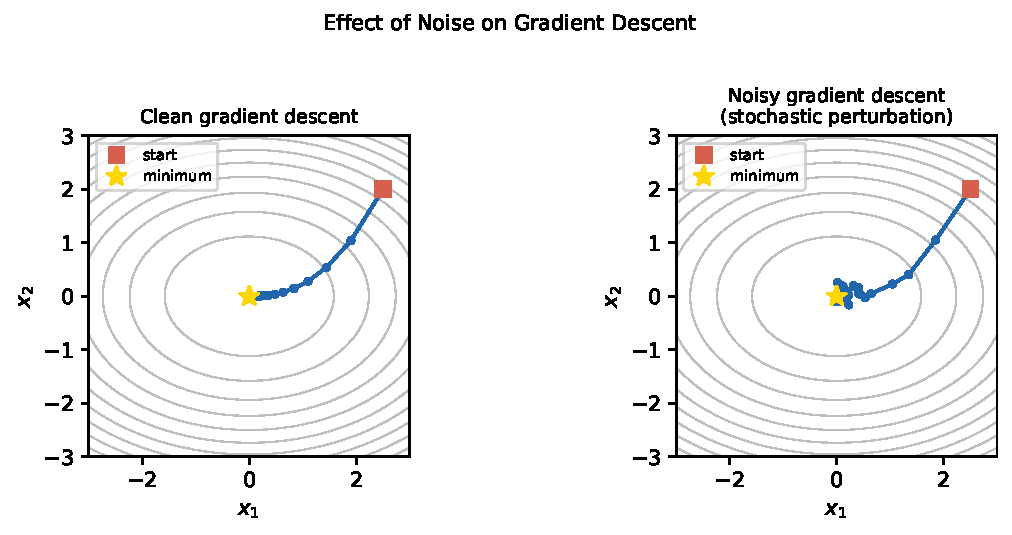
\includegraphics[width=0.55\linewidth]{noisy_descent.pdf}
\end{center}
{\small Clean versus noisy gradient descent on a quadratic bowl.
The stochastic path is jagged but can escape narrow valleys that trap the deterministic method.}

\begin{alertblock}{Key Takeaway}
Stochastic methods trade away reproducibility and smooth convergence in exchange for the ability to explore broadly and escape local optima --- a worthwhile trade-off for many real-world optimisation problems.
\end{alertblock}

\end{frame}

%%=============================================================================
\section{8.1 Noisy Descent}
%%=============================================================================

\begin{frame}[allowframebreaks]{8.1 Noisy Descent --- The Core Idea}

The simplest way to introduce randomness into gradient descent is to \emph{corrupt the gradient} with random noise at each step.
Rather than moving in the exact direction of steepest descent, we move in a direction that is close to that direction but perturbed by a random vector.
This small perturbation is enough to prevent the algorithm from getting permanently stuck, while still making overall progress toward a minimum.

\begin{block}{The Stochastic Gradient Descent (SGD) Update Rule}
At each iteration $k$ (where $k$ is the iteration counter, starting from 1), we update our current point $\mathbf{x}^{(k)}$ (read as ``x superscript k'', meaning the value of $\mathbf{x}$ at iteration number $k$) as follows:
\[
  \mathbf{x}^{(k+1)} \;\leftarrow\; \mathbf{x}^{(k)} \;-\; \alpha^{(k)}\,\tilde{\nabla} f\!\left(\mathbf{x}^{(k)}\right)
\]
\end{block}

\begin{block}{Notation}
\begin{itemize}
  \item $\mathbf{x}^{(k)}$ is our current estimate of the minimiser, a vector in $\mathbb{R}^n$ (real $n$-dimensional space).
  \item $\alpha^{(k)}$ (alpha, superscript $k$) is the \emph{step size} (also called the learning rate) at iteration $k$ --- it controls how large a step we take. A larger $\alpha$ means a bigger move.
  \item $\tilde{\nabla} f(\mathbf{x}^{(k)})$ (nabla-tilde $f$, read ``noisy gradient of $f$ at $\mathbf{x}^{(k)}$'') is a random approximation to the true gradient $\nabla f$ (nabla $f$, the vector of partial derivatives that points in the direction of steepest ascent).
  \item The minus sign means we move \emph{opposite} to the gradient --- downhill, not uphill.
\end{itemize}
The noisy gradient is defined as:
\[
  \tilde{\nabla} f(\mathbf{x}) \;=\; \nabla f(\mathbf{x}) + \boldsymbol{\epsilon}, \qquad
  \boldsymbol{\epsilon} \;\sim\; \mathcal{N}(\mathbf{0},\, \sigma^2 \mathbf{I})
\]
Here $\boldsymbol{\epsilon}$ (epsilon) is a random noise vector drawn from a multivariate Gaussian (normal) distribution with mean zero (the zero vector $\mathbf{0}$) and covariance $\sigma^2 \mathbf{I}$ (sigma squared times the identity matrix $\mathbf{I}$). The parameter $\sigma$ (sigma) controls the standard deviation --- how large the random perturbations are. Larger $\sigma$ means more noise and more exploration.
\end{block}

\begin{alertblock}{How to Read This Formula}
The update says: ``Move from your current position by a step of size $\alpha^{(k)}$ in the direction of the noisy gradient.'' Because the noise $\boldsymbol{\epsilon}$ is random, each iteration takes a slightly different direction even when $\mathbf{x}^{(k)}$ is the same. This randomness prevents the algorithm from settling permanently at a local minimum: if the noise occasionally points away from the local trap, the algorithm can escape.
\end{alertblock}

\framebreak

\begin{block}{Three Intuitive Reasons Why Noise Helps}
\begin{enumerate}
  \item \textbf{Flat regions (saddle points and plateaus).} The true gradient $\nabla f$ is nearly zero in these regions, so a deterministic method barely moves. The noise $\boldsymbol{\epsilon}$ provides a random kick that can push the algorithm out of the flat region in a direction that eventually leads downhill.

  \item \textbf{Narrow valleys.} A deterministic gradient method can oscillate back and forth across a narrow valley without making forward progress. Noise can push the algorithm along the valley floor rather than across it.

  \item \textbf{Neural-network training with mini-batches.} When the objective is an average loss over millions of data points, computing the exact gradient is expensive. Instead, we compute the gradient on a small random \emph{mini-batch} of data --- this gives a cheap, noisy estimate of the full gradient, which is exactly what SGD needs.
\end{enumerate}
\end{block}

\begin{block}{The Critical Requirement: Unbiased Gradient}
The noise must have \emph{zero mean} on average:
\[
  \mathbb{E}\!\left[\tilde{\nabla} f(\mathbf{x})\right] \;=\; \nabla f(\mathbf{x})
\]
This equation reads: ``The expected value (long-run average) of the noisy gradient equals the true gradient.'' If this condition is violated --- if the noise has a nonzero mean, i.e., it consistently pushes in a wrong direction --- the algorithm will converge to the wrong point.
\end{block}

\begin{block}{Convergence Conditions: The Robbins--Monro Requirements}
For SGD to converge to a minimum, the step sizes $\alpha^{(k)}$ must satisfy two conditions simultaneously:
\[
  \sum_{k=1}^{\infty} \alpha^{(k)} = \infty \qquad \text{and} \qquad
  \sum_{k=1}^{\infty} \left(\alpha^{(k)}\right)^2 < \infty
\]
The first condition (the sum of all step sizes is infinite) ensures that the algorithm can travel arbitrarily far --- it will always be able to \emph{reach} the minimum no matter how far away it starts. If step sizes shrank too fast, the total distance the algorithm could travel would be bounded, and it might stop short.

The second condition (the sum of squared step sizes is finite) ensures that the random fluctuations caused by the noise eventually become negligible --- the method \emph{settles down} rather than bouncing around forever.

A classic schedule that satisfies both conditions is:
\[
  \alpha^{(k)} = \frac{\alpha^{(1)}}{k}
\]
where $\alpha^{(1)}$ (alpha superscript 1) is the initial step size. For example, with $\alpha^{(1)} = 1$, the step sizes are $1, \tfrac{1}{2}, \tfrac{1}{3}, \tfrac{1}{4}, \ldots$, whose sum diverges but whose sum of squares ($1 + \tfrac{1}{4} + \tfrac{1}{9} + \cdots = \pi^2/6 \approx 1.645$) is finite.
\end{block}

\begin{exampleblock}{Worked Numerical Example}
Consider minimising $f(x_1, x_2) = x_1^2 + 2x_2^2$ starting from $\mathbf{x}^{(1)} = (3, 3)$ with step size $\alpha^{(1)} = 0.1$ and noise standard deviation $\sigma = 0.5$.

The true gradient is $\nabla f = (2x_1,\, 4x_2)$, so at $(3, 3)$ we get $\nabla f = (6, 12)$.

Suppose the noise vector at iteration 1 is $\boldsymbol{\epsilon} = (0.3, -0.2)$ (a random sample from $\mathcal{N}(\mathbf{0}, 0.25\mathbf{I})$). Then:
\[
  \tilde{\nabla} f = (6 + 0.3,\; 12 - 0.2) = (6.3,\; 11.8)
\]
\[
  \mathbf{x}^{(2)} = (3, 3) - 0.1 \times (6.3, 11.8) = (3 - 0.63,\; 3 - 1.18) = (2.37,\; 1.82)
\]
The objective drops from $f(3,3) = 9 + 18 = 27$ to $f(2.37, 1.82) = 5.62 + 6.63 = 12.25$ --- a substantial improvement in one step, despite the noise.
\end{exampleblock}

\end{frame}

\begin{frame}[fragile]{8.1 Noisy Descent --- Python Implementation}
\begin{lstlisting}[caption={Noisy gradient descent (Python/NumPy)}]
import numpy as np

def noisy_descent(f, grad_f, x0, alpha=lambda k: 1.0/k,
                  sigma=0.1, max_iter=1000, tol=1e-5):
    """
    f       : objective function  R^n -> R
    grad_f  : gradient function   R^n -> R^n
    x0      : initial point
    alpha   : step-size schedule  k -> float  (default: 1/k)
    sigma   : noise standard deviation (controls exploration)
    """
    x = np.array(x0, dtype=float)
    for k in range(1, max_iter + 1):
        g     = grad_f(x)                        # true gradient
        noise = np.random.randn(len(x)) * sigma  # random perturbation
        g_hat = g + noise                        # noisy gradient
        x     = x - alpha(k) * g_hat            # SGD update
        if np.linalg.norm(alpha(k) * g_hat) < tol:
            break
    return x

# Example: minimize f(x) = x1^2 + 2*x2^2  from x0 = [3, 3]
f      = lambda x: x[0]**2 + 2*x[1]**2
grad_f = lambda x: np.array([2*x[0], 4*x[1]])
x_opt  = noisy_descent(f, grad_f, [3.0, 3.0], sigma=0.5)
print(f"Optimum: {x_opt}")   # approx [0, 0]
\end{lstlisting}
\end{frame}

%%=============================================================================
\section{8.2 Mesh Adaptive Direct Search (MADS)}
%%=============================================================================

\begin{frame}[allowframebreaks]{8.2 Mesh Adaptive Direct Search (MADS)}

Mesh Adaptive Direct Search (MADS) is a \emph{zeroth-order} method, meaning it requires only function values $f(\mathbf{x})$ --- no gradients.
This makes it ideal for \emph{black-box} problems where the objective is computed by a simulation or a legacy code that provides no derivative information.

The core idea is to systematically probe a set of search directions around the current point.
If any direction produces an improvement, we move there and expand our step size; if none do, we shrink the step size and try again with a finer mesh.
The randomness enters through how the search directions are generated at each iteration.

\begin{block}{What is a Positive Spanning Set?}
A set of vectors $\{\mathbf{d}^{(1)}, \ldots, \mathbf{d}^{(n+1)}\}$ is called a \emph{positive spanning set} if every direction in $\mathbb{R}^n$ can be written as a \emph{non-negative} combination of these vectors.
Intuitively, the vectors ``point in all directions'' --- they collectively cover the entire space, so no descent direction can be missed by the search.

For $n = 2$ (two-dimensional problems), a positive spanning set consists of at least 3 vectors; MADS uses $n+1 = 3$ vectors in 2D and $n+1$ vectors in general.
\end{block}

\begin{block}{Algorithm: Generating a Random Positive Spanning Set}
MADS uses a random lower-triangular matrix to generate its search directions. The procedure is:
\begin{enumerate}
  \item Compute the mesh granularity parameter $\delta$ (delta, a positive integer) from the current step size $\alpha$ (alpha):
    \[
      \delta = \left\lfloor \frac{1}{\sqrt{\alpha}} \right\rfloor
    \]
    Here $\lfloor \cdot \rfloor$ (floor) means round down to the nearest integer. As $\alpha$ (alpha) decreases, $\delta$ increases, making the search directions more varied and the mesh finer.

  \item Build a random lower-triangular matrix $\mathbf{L}$ (capital L) of size $n \times n$:
    \begin{itemize}
      \item The diagonal entries are randomly $+1$ or $-1$.
      \item The below-diagonal entries are random integers in $\{-\delta+1, \ldots, \delta-1\}$.
      \item Upper-triangular entries are zero.
    \end{itemize}

  \item Randomly permute the rows and columns of $\mathbf{L}$ to obtain $\mathbf{D}$ (capital D). This permutation ensures that no single coordinate is always probed first, making the search direction selection unbiased.

  \item Add one extra direction $\mathbf{d}^{(n+1)} = -\sum_{i=1}^{n} \mathbf{d}^{(i)}$, which is the negative sum of all previous directions. This extra direction guarantees the positive spanning property.
\end{enumerate}
\end{block}

\begin{center}
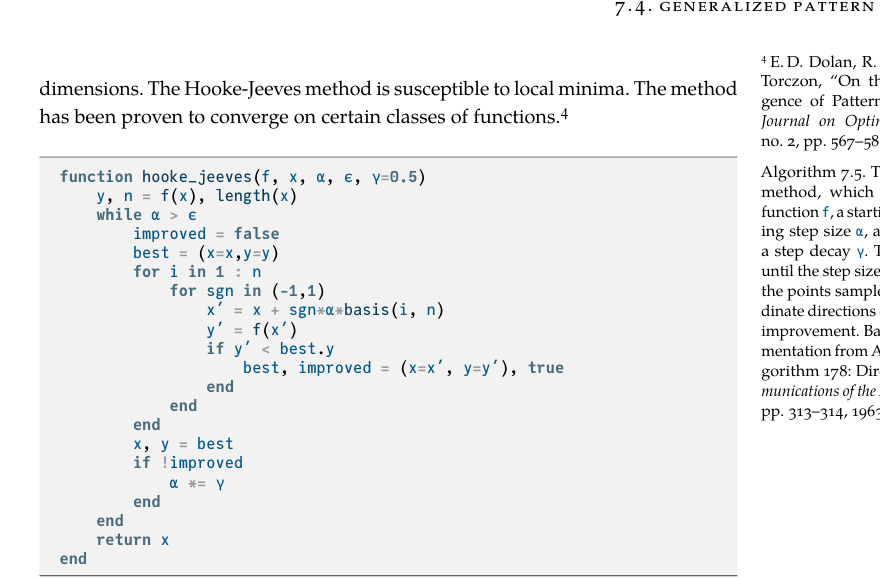
\includegraphics[width=0.65\linewidth]{book_mads_spanning.png}
\end{center}
{\small \textbf{Example 8.1.} Eight different positive spanning sets for $\mathbb{R}^2$, each generated by the random lower-triangular construction. Only this construction can produce the first two columns shown (directions that are not axis-aligned).}

\framebreak

\begin{block}{The MADS Step-Size Update Rule}
After generating the spanning set, MADS evaluates $f$ at $\mathbf{x} + \alpha \mathbf{d}$ for each direction $\mathbf{d}$ in the spanning set:
\begin{enumerate}
  \item If any direction produces $f(\mathbf{x} + \alpha \mathbf{d}) < f(\mathbf{x})$ (an improvement), we:
    \begin{itemize}
      \item Accept the new point $\mathbf{x}' = \mathbf{x} + \alpha \mathbf{d}$.
      \item Also probe an \emph{opportunistic} extended step $\mathbf{x}'' = \mathbf{x} + 3\alpha\mathbf{d}$ --- if this is even better, take it instead.
      \item Mark \texttt{improved = True} and stop probing other directions.
    \end{itemize}
  \item Update the step size $\alpha$ (alpha) according to:
    \[
      \alpha^{(k+1)} \;\leftarrow\;
      \begin{cases}
        \min\!\left(1,\; 4\alpha^{(k)}\right) & \text{if an improvement was found} \\[4pt]
        \alpha^{(k)} / 4 & \text{if no improvement was found}
      \end{cases}
    \]
\end{enumerate}
\end{block}

\begin{block}{Notation for the Step-Size Rule}
\begin{itemize}
  \item $\alpha^{(k)}$ (alpha superscript $k$) is the step size at iteration $k$. It always remains a power of $\tfrac{1}{4}$: $\alpha \in \{1, \tfrac{1}{4}, \tfrac{1}{16}, \tfrac{1}{64}, \ldots\}$.
  \item Multiplying by 4 when we improve is aggressive expansion --- we have found a good direction and want to exploit it.
  \item Dividing by 4 when we fail is cautious contraction --- the minimum must be closer than we thought, so we refine the mesh.
  \item The $\min(1, \cdot)$ cap ensures the step size never exceeds 1.
\end{itemize}
\end{block}

\begin{alertblock}{Key Insight: Why Powers of Four?}
Because $\alpha$ is always a power of $\tfrac{1}{4} = 4^{-m}$ for some non-negative integer $m$, the quantity $\sqrt{\alpha} = 2^{-m}$ is always a power of $\tfrac{1}{2}$.
This means the maximum componentwise step size $\alpha \cdot \|\mathbf{d}\|_\infty = \alpha / \sqrt{\alpha} = \sqrt{\alpha}$ lies on a dyadic grid (a grid with spacings that are powers of 2).
As $\alpha \to 0$, this grid becomes arbitrarily fine, which is the key property that guarantees the algorithm eventually finds directions of descent and converges.
\end{alertblock}

\begin{columns}[T]
\column{0.50\textwidth}
\begin{block}{Summary of Properties}
MADS has four important properties that make it practical:
\begin{itemize}
  \item \textbf{Convergence is guaranteed} as $\alpha \to 0$ because the spanning sets become dense (they cover all directions with arbitrarily fine resolution).
  \item \textbf{No gradient is required} --- the method is purely zeroth-order, suitable for black-box problems.
  \item \textbf{Opportunistic evaluation} means the algorithm immediately exploits a promising direction rather than exhaustively checking all directions first.
  \item \textbf{Practical for noisy objectives} because the step-size mechanism naturally smooths over small fluctuations.
\end{itemize}
\end{block}
\column{0.47\textwidth}
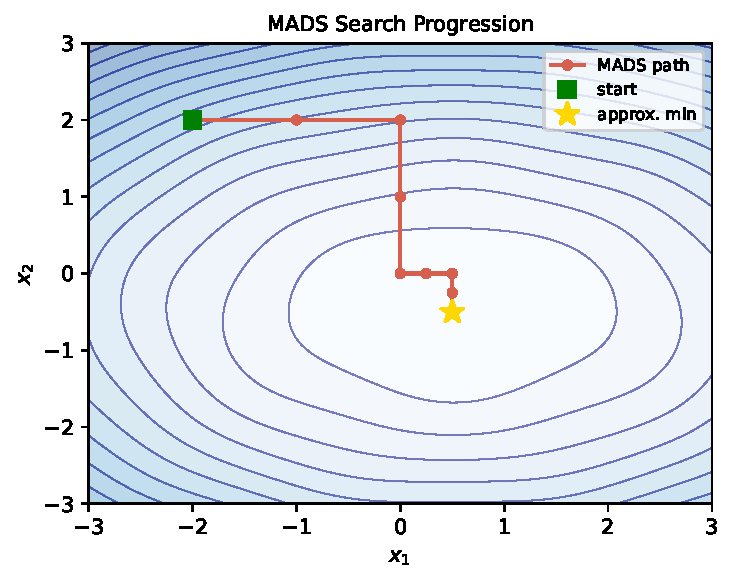
\includegraphics[width=\linewidth]{mads_search.pdf}
{\small A MADS trajectory on a noisy quadratic function. The step size expands when progress is made and contracts when the search stalls.}
\end{columns}

\end{frame}

\begin{frame}[fragile]{8.2 MADS --- Python Implementation}
\begin{lstlisting}[caption={MADS: random positive spanning set + search (Algorithms 8.2 and 8.3)}]
import numpy as np

def rand_positive_spanning_set(alpha, n):
    """Algorithm 8.2: random positive spanning set of n+1 directions."""
    delta = int(round(1 / np.sqrt(alpha)))
    L = np.diag(np.random.choice([-1, 1], n))       # diagonal +/-1
    for i in range(1, n):
        for j in range(i):
            L[i, j] = np.random.randint(-delta+1, delta)  # subdiagonal
    perm_r = np.random.permutation(n)
    perm_c = np.random.permutation(n)
    D = L[perm_r, :][:, perm_c]
    extra = -D.sum(axis=1, keepdims=True)            # -(sum of columns)
    return np.hstack([D, extra]).T                   # shape (n+1, n)

def mesh_adaptive_direct_search(f, x, eps=1e-4, alpha_init=1.0):
    """Algorithm 8.3: MADS."""
    alpha, y, n = alpha_init, f(x), len(x)
    while alpha > eps:
        improved = False
        for d in rand_positive_spanning_set(alpha, n):
            x_new = x + alpha * d;  y_new = f(x_new)
            if y_new < y:
                x, y, improved = x_new, y_new, True
                x2 = x + 3*alpha*d;  y2 = f(x2)   # opportunistic probe
                if y2 < y:  x, y = x2, y2
                break
        alpha = min(4*alpha, 1.0) if improved else alpha / 4
    return x

# Usage: minimize f(x,y) = (x-1)^2 + 2*(y+1)^2
f = lambda x: (x[0]-1)**2 + 2*(x[1]+1)**2
print(mesh_adaptive_direct_search(f, np.array([3.0, 3.0])))  # -> [1, -1]
\end{lstlisting}
\end{frame}

%%=============================================================================
\section{8.3 Memory-Efficient Zeroth-Order Optimization (MeZO)}
%%=============================================================================

\begin{frame}[allowframebreaks]{8.3 Memory-Efficient Zeroth-Order Optimization (MeZO)}

Training or fine-tuning a large language model (LLM) with billions of parameters requires not only storing the parameters themselves but also storing the \emph{gradient} of every parameter --- and, during backpropagation, the \emph{intermediate activations} at every layer.
For a model with $n$ parameters, this means roughly $3n$ to $5n$ floating-point numbers must be held in memory simultaneously, which can easily exceed the memory of available hardware.

MeZO (Memory-Efficient Zeroth-Order, Zhang et al.\ 2022) solves this problem by \emph{estimating} the gradient using only two forward passes through the model, requiring $O(1)$ extra memory beyond the parameters themselves.
The trick is to use a \emph{pseudo-random number generator (PRNG) with a fixed seed} to generate the random direction, so we can re-generate the same direction for the parameter update without ever storing it.

\begin{block}{The MeZO Gradient Estimator}
At each step, MeZO samples a random unit direction $\mathbf{z}$ (z, a random vector) from a standard multivariate Gaussian distribution, using a fixed PRNG seed $s$:
\[
  \mathbf{z} \;\sim\; \mathcal{N}(\mathbf{0},\, \mathbf{I})
\]
It then evaluates the objective at two nearby points and computes a \emph{finite-difference gradient estimate}:
\[
  \hat{g} \;=\; \frac{f(\mathbf{x} + \varepsilon\mathbf{z}) - f(\mathbf{x} - \varepsilon\mathbf{z})}{2\varepsilon}\;\mathbf{z}
\]
The parameter update is then:
\[
  \mathbf{x} \;\leftarrow\; \mathbf{x} - \alpha\,\hat{g}
\]
\end{block}

\begin{block}{Notation}
\begin{itemize}
  \item $\varepsilon$ (epsilon) is the \emph{smoothing radius} --- how far we perturb $\mathbf{x}$ in the direction $\mathbf{z}$ to probe the function. A smaller $\varepsilon$ gives a more accurate finite-difference estimate but is more sensitive to numerical noise; a larger $\varepsilon$ is more robust but less accurate.
  \item $\mathbf{z}$ (z) is the random direction vector, the same dimension as $\mathbf{x}$. Because $\mathbf{z} \sim \mathcal{N}(\mathbf{0}, \mathbf{I})$, it is isotropic --- it points in a random direction in the full $n$-dimensional space.
  \item $f(\mathbf{x} + \varepsilon\mathbf{z})$ is a forward pass through the model at a slightly perturbed parameter set. No backward pass (backpropagation) is needed.
  \item $\hat{g}$ (g-hat) is the gradient estimate. It is a scalar times $\mathbf{z}$, so it always points along the random direction $\mathbf{z}$.
  \item $\alpha$ (alpha) is the learning rate (step size).
\end{itemize}
\end{block}

\begin{alertblock}{How to Read This Formula}
The fraction $\frac{f(\mathbf{x} + \varepsilon\mathbf{z}) - f(\mathbf{x} - \varepsilon\mathbf{z})}{2\varepsilon}$ is the \emph{directional derivative} of $f$ along $\mathbf{z}$, approximated by finite differences. Multiplying by $\mathbf{z}$ converts this scalar directional derivative into a vector that estimates the full gradient. The key insight is that $\mathbb{E}[\hat{g}] = \nabla f(\mathbf{x})$ --- averaged over many random directions $\mathbf{z}$, this estimate is unbiased.
\end{alertblock}

\begin{block}{The Memory Trick: PRNG Seeds}
After computing $\hat{g}$, we need to perform the update $\mathbf{x} \leftarrow \mathbf{x} - \alpha \hat{g}$.
This requires knowing $\mathbf{z}$ again.
Instead of storing $\mathbf{z}$ (which would require $O(n)$ memory), we \emph{re-initialise} the PRNG with the same seed $s$ and regenerate $\mathbf{z}$ from scratch.
Since a PRNG always produces the same sequence from the same seed, we get the identical vector $\mathbf{z}$ without any extra storage.
The update then modifies each parameter $x_i$ by $-\alpha \cdot \hat{g}_\text{scalar} \cdot z_i$, computed one element at a time, requiring only $O(1)$ extra memory regardless of model size.
\end{block}

\begin{exampleblock}{Worked Numerical Example (One Dimension)}
Consider $f(x) = x^2$, starting at $x_0 = 3$, with $\varepsilon = 0.3$ and $\alpha = 0.1$.

The random direction in 1D is just a scalar $z$. Suppose $z = 1$ (drawn from the standard normal).

\begin{align*}
  f(x_0 + \varepsilon z) &= f(3 + 0.3 \times 1) = f(3.3) = 10.89 \\
  f(x_0 - \varepsilon z) &= f(3 - 0.3 \times 1) = f(2.7) = 7.29 \\
  \hat{g}_\text{scalar} &= \frac{10.89 - 7.29}{2 \times 0.3} = \frac{3.6}{0.6} = 6.0
\end{align*}

The true gradient at $x = 3$ is $f'(3) = 2 \times 3 = 6$. The estimate is exact here because $f(x) = x^2$ is quadratic and the central-difference formula is exact for polynomials up to degree 2.

The update: $x_1 = 3 - 0.1 \times 6.0 \times 1 = 3 - 0.6 = 2.4$.
\end{exampleblock}

\begin{block}{Key Properties of MeZO}
\begin{itemize}
  \item \textbf{Memory usage:} $O(1)$ extra memory beyond the model parameters --- just two scalar function values and a seed.
  \item \textbf{Unbiasedness:} $\mathbb{E}[\hat{g}] = \nabla f(\mathbf{x})$ by the spherical symmetry of the Gaussian distribution.
  \item \textbf{No backward pass:} Only two forward passes are needed per update, which is possible even for models that are not differentiable or where the backward pass is unavailable.
  \item \textbf{Best suited for fine-tuning:} MeZO works well when the model is already close to a good solution (e.g., a pretrained LLM being fine-tuned on a new task). It is not a general replacement for SGD when training from scratch on large datasets.
\end{itemize}
\end{block}

\end{frame}

\begin{frame}[fragile]{8.3 MeZO --- Python Implementation}
\begin{lstlisting}[caption={MeZO: memory-efficient zeroth-order optimisation (Algorithm 8.4)}]
import numpy as np

def mezo_step(f, x, eps=1e-3, alpha=1e-3, seed=None):
    """
    One MeZO step. Re-uses PRNG seed to avoid storing z.
    f    : objective (x -> scalar)
    x    : current parameters (modified in place)
    eps  : smoothing radius (epsilon)
    alpha: learning rate
    """
    rng = np.random.default_rng(seed)
    z = rng.standard_normal(x.shape)          # random direction
    # Two function evaluations (forward passes only)
    f_plus  = f(x + eps * z)
    f_minus = f(x - eps * z)
    grad_est = (f_plus - f_minus) / (2 * eps)  # scalar directional derivative
    # Re-generate same z using same seed for in-place update
    rng2 = np.random.default_rng(seed)
    z2   = rng2.standard_normal(x.shape)
    x -= alpha * grad_est * z2                 # O(1) extra memory
    return x

def mezo_optimize(f, x0, n_iter=500, eps=1e-3, alpha=1e-3):
    x = np.array(x0, dtype=float)
    for k in range(n_iter):
        x = mezo_step(f, x, eps=eps, alpha=alpha, seed=k)
    return x

# Fine-tuning demo on a simple quadratic
f_quad = lambda x: np.sum((x - np.array([1.0, 2.0]))**2)
x_opt  = mezo_optimize(f_quad, [5.0, 5.0], n_iter=2000, alpha=0.05)
print(f"Solution: {x_opt}")   # approaches [1, 2]
\end{lstlisting}
\end{frame}

%%=============================================================================
\section{8.4 Simulated Annealing}
%%=============================================================================

\begin{frame}[allowframebreaks]{8.4 Simulated Annealing --- Core Idea}

Simulated annealing (SA) is inspired by a physical process from metallurgy: when a metal is heated to a high temperature and then slowly cooled (\emph{annealed}), its atoms settle into a low-energy crystalline structure.
If the cooling is too fast, atoms get trapped in disordered, high-energy configurations --- the physical analogue of a local minimum.
If the cooling is slow and controlled, the system finds its global minimum energy state.

In optimisation, the ``temperature'' $t$ (t) is a control parameter that governs how willing we are to accept a worse solution. At high temperature, we accept almost any move --- we explore broadly. As temperature decreases, we become increasingly selective, accepting only moves that improve the objective. This smooth transition from exploration to exploitation is what allows SA to escape local minima early in the search and converge to a good solution later.

\begin{block}{The Metropolis Acceptance Criterion}
At each iteration $k$, we propose a new point $\mathbf{x}'$ drawn from a transition distribution $T(\mathbf{x}'|\mathbf{x}^{(k)})$, which is typically a Gaussian centred at $\mathbf{x}^{(k)}$.
We then decide whether to accept or reject $\mathbf{x}'$ using the following rule:
\[
  \mathbf{x}^{(k+1)} \;\leftarrow\;
  \begin{cases}
    \mathbf{x}' & \text{if } f(\mathbf{x}') \le f(\mathbf{x}^{(k)}) \quad \text{(always accept improvements)} \\[4pt]
    \mathbf{x}' & \text{with probability } e^{-\Delta y / t^{(k)}} \quad \text{(sometimes accept worsening)} \\[4pt]
    \mathbf{x}^{(k)} & \text{otherwise (stay in place)}
  \end{cases}
\]
where $\Delta y = f(\mathbf{x}') - f(\mathbf{x}^{(k)}) > 0$ is the amount by which the proposed point is \emph{worse}.
\end{block}

\begin{block}{Notation}
\begin{itemize}
  \item $t^{(k)}$ (t superscript $k$) is the \emph{temperature} at iteration $k$. It is a positive real number that decreases over time according to a \emph{cooling schedule}.
  \item $\Delta y$ (Delta y, where $\Delta$ (Delta) means ``change in'') is the increase in objective value from accepting the proposed point. Since we are minimising, $\Delta y > 0$ means the proposed point is worse.
  \item $e^{-\Delta y / t^{(k)}}$ (e to the power of negative Delta-y over t-k) is the \emph{acceptance probability} for a worsening move. Here $e \approx 2.718$ is Euler's number.
\end{itemize}
\end{block}

\begin{alertblock}{How to Read the Acceptance Probability}
The formula $e^{-\Delta y / t}$ is always between 0 and 1 (since $\Delta y > 0$ and $t > 0$), so it is a valid probability. Two things determine this probability:
\begin{itemize}
  \item \textbf{How bad is the proposed move ($\Delta y$)?} A small $\Delta y$ (slightly worse) gives a high acceptance probability; a large $\Delta y$ (much worse) gives a very low acceptance probability. This is sensible --- we are more likely to accept a small setback than a catastrophic one.
  \item \textbf{What is the temperature ($t$)?} At high $t$, $e^{-\Delta y / t} \approx 1$ and almost everything is accepted. At low $t$, $e^{-\Delta y / t} \approx 0$ and only improvements are accepted.
\end{itemize}
This is directly analogous to the physical process: a hot metal atom can easily overcome an energy barrier, while a cold atom is unlikely to.
\end{alertblock}

\begin{columns}[T]
\column{0.55\textwidth}
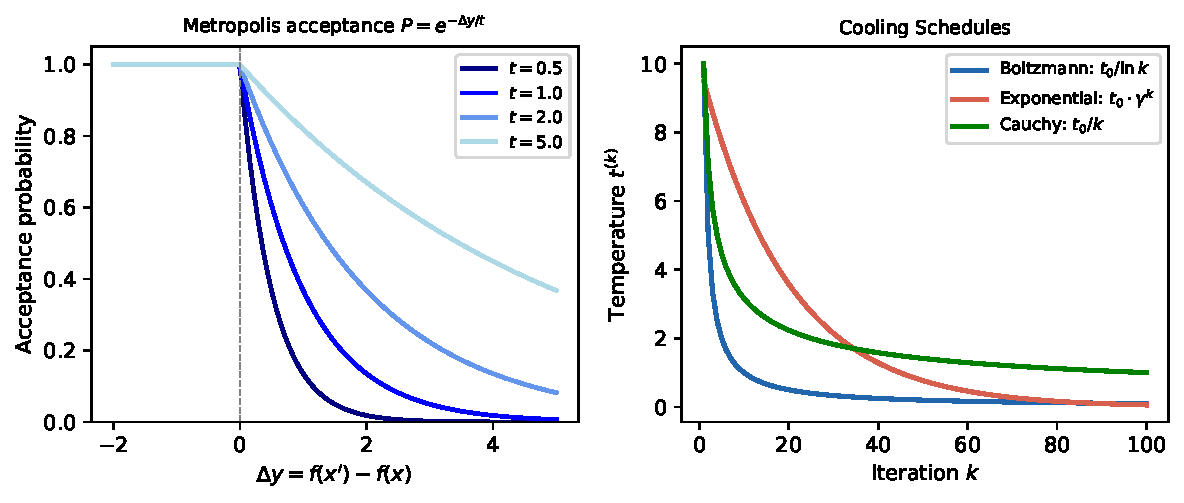
\includegraphics[width=\linewidth]{sa_acceptance.pdf}
\column{0.42\textwidth}
{\small \textbf{Left:} Acceptance probability $e^{-\Delta y / t}$ as a function of $\Delta y$ (the amount the proposed point is worse) for various temperatures $t$. At high $t$, the curve is flat near 1 (everything accepted); at low $t$, it drops sharply to 0. \textbf{Right:} Three standard cooling schedules showing how $t$ decreases over iterations.}
\end{columns}

\framebreak

\begin{block}{Standard Cooling Schedules}
The cooling schedule determines how the temperature $t^{(k)}$ decreases from iteration to iteration. Three standard choices are:

\medskip
\begin{center}
\begin{tabular}{llll}
\toprule
Name & Formula & Convergence & Comment \\
\midrule
Boltzmann & $t^{(k)} = t^{(1)} / \ln(k)$ & Asymptotically guaranteed & Very slow \\
Cauchy & $t^{(k)} = t^{(1)} / k$ & Guaranteed under conditions & Faster \\
Exponential & $t^{(k)} = t^{(1)} \cdot \gamma^k$ & Not guaranteed & Most practical \\
\bottomrule
\end{tabular}
\end{center}
\medskip
Here $t^{(1)}$ (t superscript 1) is the initial temperature, $\ln(\cdot)$ (ln) denotes the natural logarithm, and $\gamma$ (gamma) is a constant slightly less than 1 (such as $\gamma = 0.95$) for the exponential schedule.
\end{block}

\begin{block}{Boltzmann Annealing: Slow but Theoretically Sound}
The Boltzmann schedule pairs with a \emph{Gaussian} transition distribution: we propose $\mathbf{x}' = \mathbf{x} + t^{(k)} \mathcal{N}(\mathbf{0}, \mathbf{I})$.
The proposal spread shrinks with temperature, which together with the $1/\ln(k)$ cooling guarantees that the method converges to the global minimum --- but only \emph{asymptotically} (as $k \to \infty$), which in practice can require an impractically large number of iterations.
\end{block}

\begin{block}{Fast Simulated Annealing (Cauchy Schedule)}
The Cauchy/Lorentz transition distribution has \emph{heavier tails} than the Gaussian: very large jumps are much more likely.
This allows the algorithm to explore widely even at moderate temperatures.
The schedule $t^{(k)} = t^{(1)}/k$ cools faster than Boltzmann but is still slow enough that, under certain conditions, global convergence is maintained.
\end{block}

\begin{exampleblock}{Exponential Cooling: A Numerical Table}
With $t^{(1)} = 10$ and $\gamma = 0.95$ (ninety-five percent of the previous temperature), the temperatures at selected iterations are:
\begin{center}
\begin{tabular}{rr}
\toprule
Iteration $k$ & Temperature $t^{(k)} = 10 \times 0.95^k$ \\
\midrule
1   & 9.50 \\
10  & 5.99 \\
50  & 0.769 \\
100 & 0.059 \\
200 & 0.00035 \\
\bottomrule
\end{tabular}
\end{center}
At $t = 1$, the probability of accepting a move that is 1 unit worse is $e^{-1/1} \approx 0.368$ (about 37\%), and the probability of accepting a move that is 5 units worse is $e^{-5/1} \approx 0.007$ (about 0.7\%). At $t = 0.001$, even a move that is 0.01 units worse has acceptance probability $e^{-10} \approx 0.00005$ --- effectively never accepted.
\end{exampleblock}

\end{frame}

\begin{frame}[fragile]{8.4 Simulated Annealing --- Python Implementation}
\begin{lstlisting}[caption={Simulated annealing (Algorithm 8.6)}]
import numpy as np

def simulated_annealing(f, x0, t_init=10.0, t_schedule='boltzmann',
                        sigma=1.0, n_iter=1000):
    """
    f          : objective function
    x0         : starting point
    t_init     : initial temperature
    t_schedule : 'boltzmann' | 'cauchy' | 'exponential'
    sigma      : transition distribution std. dev.
    """
    x = np.array(x0, dtype=float)
    y = f(x)
    best_x, best_y = x.copy(), y
    gamma = 0.95  # for exponential schedule

    for k in range(1, n_iter + 1):
        # Temperature schedule
        if t_schedule == 'boltzmann':
            t = t_init / np.log(k + 1)
        elif t_schedule == 'cauchy':
            t = t_init / k
        else:  # exponential
            t = t_init * gamma**k

        # Propose new point (Gaussian transition)
        x_new = x + np.random.randn(len(x)) * sigma
        y_new = f(x_new)
        delta = y_new - y

        # Metropolis acceptance
        if delta < 0 or np.random.rand() < np.exp(-delta / max(t, 1e-12)):
            x, y = x_new, y_new
            if y < best_y:
                best_x, best_y = x.copy(), y

    return best_x

# Minimize Ackley function (has many local minima)
def ackley(x, a=20, b=0.2, c=2*np.pi):
    n = len(x)
    return (-a*np.exp(-b*np.sqrt(np.sum(x**2)/n))
            - np.exp(np.sum(np.cos(c*x))/n) + a + np.e)

x_opt = simulated_annealing(ackley, [15.0, 15.0], sigma=5.0, n_iter=5000)
print(f"SA result: {x_opt}, f={ackley(x_opt):.4f}")  # near [0,0]
\end{lstlisting}
\end{frame}

\begin{frame}[allowframebreaks]{8.4 SA --- Effect of Temperature and Variance (Example 8.2)}

The Ackley function is a classic benchmark with many local minima arranged in a highly irregular landscape. It has a global minimum of 0 at $\mathbf{x} = \mathbf{0}$, surrounded by many local minima that can trap gradient-based methods.

\begin{columns}[T]
\column{0.48\textwidth}
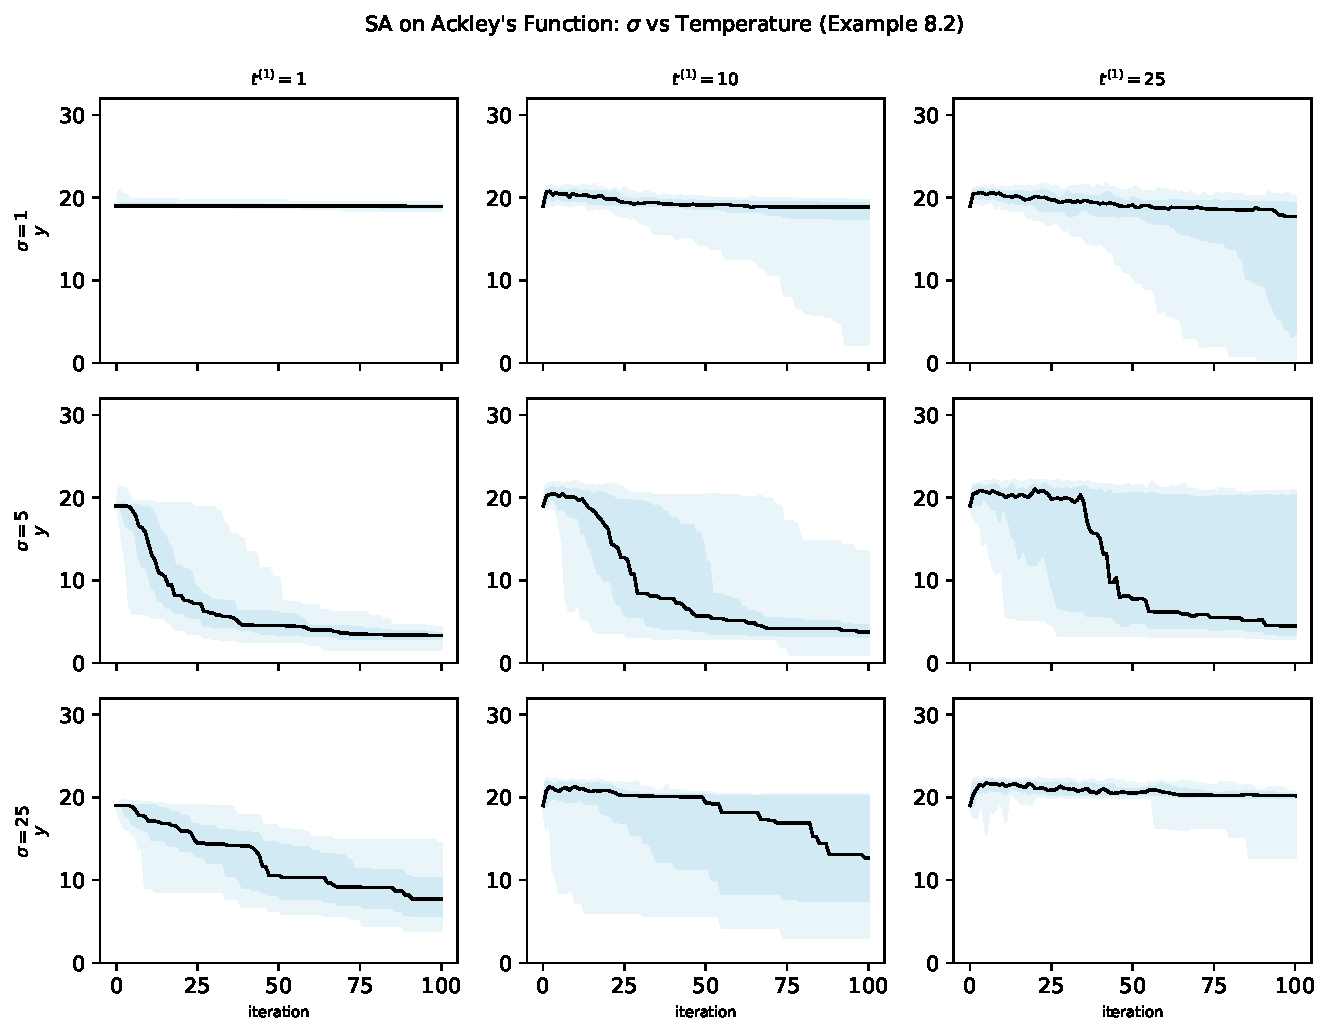
\includegraphics[width=\linewidth]{sa_ackley.pdf}
\column{0.49\textwidth}
\begin{block}{What the Experiment Shows}
The key variable is the standard deviation $\sigma$ (sigma) of the Gaussian transition distribution --- it controls how far the algorithm can jump in a single step.

\begin{itemize}
  \item \textbf{Small $\sigma = 1$:} The algorithm can only make small moves. Local minima near the starting point will trap it, because the probability of jumping over the barrier to a better minimum is negligible.

  \item \textbf{Large $\sigma = 25$:} The algorithm makes very large, essentially random jumps. It explores broadly but wastes most of its function evaluations on points far from any minimum. Convergence is extremely slow.

  \item \textbf{Optimal $\sigma \approx 5$:} The spread is large enough to jump between nearby local minima but small enough that many evaluations land in productive regions. This balance gives the best final solution quality.

  \item \textbf{Temperature schedule:} On the Ackley function, the choice of cooling schedule (Boltzmann, Cauchy, exponential) has a \emph{secondary} effect compared to the spread $\sigma$. Getting the transition distribution right is more important than the exact cooling rate.
\end{itemize}
\end{block}
\end{columns}

\begin{alertblock}{Key Takeaway}
For functions with widely-separated local minima, match the transition distribution spread to the typical distance between minima. The temperature schedule controls \emph{when} to stop exploring; the spread controls \emph{how far} you can explore in each step.
\end{alertblock}

\end{frame}

\begin{frame}[allowframebreaks]{8.4 Adaptive Simulated Annealing (Algorithm 8.7)}

Standard SA uses the same step distribution for all coordinates, which is inefficient when the function varies at very different scales in different directions.
Adaptive SA (Ingber, 1989) assigns each coordinate $i$ its own step vector $v_i$ and adjusts it so that the acceptance rate in that direction stays near 50\%.

\begin{block}{The Adaptive SA Procedure}
\begin{enumerate}
  \item Run a \emph{cycle} of $n_s$ random moves, varying one coordinate at a time.
  \item Count $A_i$ = number of accepted moves in coordinate direction $i$.
  \item Adjust the step size $v_i$ (v sub i) for each coordinate:
    \[
      v_i \;\leftarrow\;
      \begin{cases}
        v_i\!\left(1 + c_i\dfrac{A_i/n_s - 0.6}{0.4}\right)
          & \text{if } A_i > 0.6\,n_s \quad \text{(accept rate too high, increase step)} \\[8pt]
        v_i\!\left(1 + c_i\dfrac{0.4 - A_i/n_s}{0.4}\right)^{-1}
          & \text{if } A_i < 0.4\,n_s \quad \text{(accept rate too low, decrease step)} \\[8pt]
        v_i & \text{otherwise \quad (accept rate in target range)}
      \end{cases}
    \]
  \item Repeat for $n_t$ temperature-reduction cycles, then lower the temperature.
  \item When no adjustment is needed for $n_\varepsilon$ consecutive cycles, add the current point to the list of candidate optima.
\end{enumerate}
\end{block}

\begin{block}{Notation}
\begin{itemize}
  \item $v_i$ (v sub i) is the step size for coordinate $i$. Different coordinates can have very different step sizes, which is the key advantage over standard SA.
  \item $A_i$ (A sub i) is the number of accepted moves out of $n_s$ (n sub s) attempts in direction $i$.
  \item $A_i / n_s$ is the empirical acceptance rate, which we target to be between 0.4 and 0.6 (40\% to 60\%).
  \item $c_i$ (c sub i) is a tuning constant (typically $c_i = 2$) that controls how aggressively the step size is adjusted.
\end{itemize}
\end{block}

\begin{alertblock}{Why Target 50\% Acceptance?}
A 50\% acceptance rate balances exploration and exploitation: if almost all moves are accepted, the step is too small and the algorithm is not exploiting the objective; if almost no moves are accepted, the step is too large and the algorithm is wasting evaluations on proposals that will always be rejected.
\end{alertblock}

\begin{center}
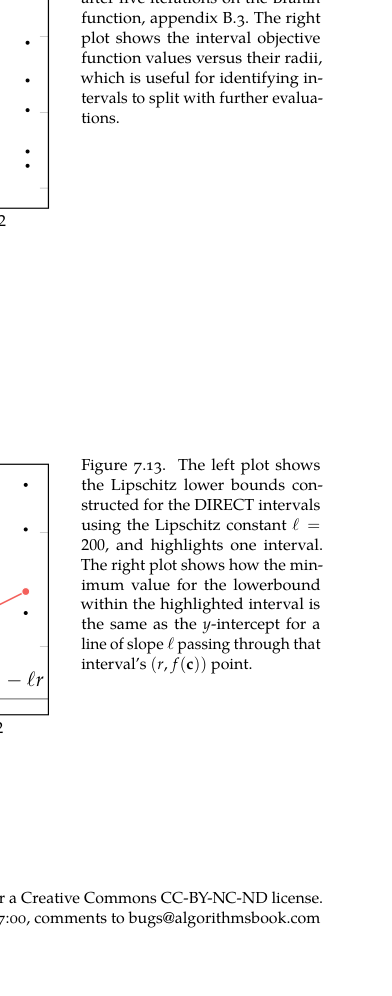
\includegraphics[width=0.55\linewidth]{book_sa_flowchart.png}
\end{center}
{\small Flowchart of the adaptive simulated annealing algorithm, showing the nested loops: inner loop over coordinate moves, middle loop over temperature-reduction cycles, and outer loop checking the termination condition.}

\end{frame}

%%=============================================================================
\section{8.5 Cross-Entropy Method}
%%=============================================================================

\begin{frame}[allowframebreaks]{8.5 Cross-Entropy Method}

The Cross-Entropy Method (CEM) takes a fundamentally different approach to optimisation: instead of maintaining a single current point, it maintains a \emph{probability distribution} over the design space.
The distribution is iteratively updated to concentrate probability mass near the best solutions found so far.
Ultimately, the distribution collapses onto the global minimum.

The name ``cross-entropy'' comes from information theory: the algorithm minimises the cross-entropy between the current proposal distribution and an ideal target distribution concentrated at the global minimum. In practice, we achieve this by fitting the distribution to the \emph{elite samples} --- the best-performing subset of samples drawn from the current distribution.

\begin{block}{The CEM Algorithm}
\begin{enumerate}
  \item \textbf{Sample:} Draw $m$ (m) candidate solutions $\mathbf{x}^{(1)}, \ldots, \mathbf{x}^{(m)}$ from the current proposal distribution $P_\theta(\mathbf{x})$, where $\theta$ (theta) are the distribution parameters (e.g., mean and covariance for a Gaussian).
  \item \textbf{Evaluate and rank:} Compute $f(\mathbf{x}^{(i)})$ for each sample and rank the samples from best (lowest $f$) to worst. Select the top $m_\text{elite}$ (m subscript ``elite'') samples as the \emph{elite set} $\mathcal{E}$.
  \item \textbf{Refit:} Update $P_\theta$ by fitting it to the elite set using maximum likelihood estimation (MLE). For a Gaussian distribution, MLE gives the sample mean and covariance of the elite set.
  \item \textbf{Repeat} until the distribution is sufficiently concentrated (e.g., standard deviation below a threshold).
\end{enumerate}
\end{block}

\begin{block}{MLE Update Formulas for a Gaussian Proposal $\mathcal{N}(\bm{\mu}, \bm{\Sigma})$}
After selecting the $m_e$ (m sub e) elite samples $\{\mathbf{x}^{(i)}\}_{i=1}^{m_e}$, we update the distribution parameters by:
\[
  \bm{\mu}^{(k+1)} \;=\; \frac{1}{m_e}\sum_{i=1}^{m_e}\mathbf{x}^{(i)}
\]
\[
  \bm{\Sigma}^{(k+1)} \;=\; \frac{1}{m_e}\sum_{i=1}^{m_e}\!\left(\mathbf{x}^{(i)}-\bm{\mu}^{(k+1)}\right)\!\left(\mathbf{x}^{(i)}-\bm{\mu}^{(k+1)}\right)^\top
\]
\end{block}

\begin{block}{Notation for the MLE Updates}
\begin{itemize}
  \item $\bm{\mu}^{(k+1)}$ (bold mu, superscript $k+1$) is the new mean vector of the proposal distribution. It is the arithmetic average (centroid) of the elite samples.
  \item $\bm{\Sigma}^{(k+1)}$ (bold Sigma, superscript $k+1$) is the new covariance matrix. Each term $(\mathbf{x}^{(i)} - \bm{\mu})(\mathbf{x}^{(i)} - \bm{\mu})^\top$ is an outer product (a matrix formed from a column vector times its own transpose), and we average these over all elite samples.
  \item $\Sigma$ (Sigma) is an $n \times n$ symmetric positive-definite matrix that encodes both the variances of each coordinate and the correlations between coordinates.
\end{itemize}
\end{block}

\begin{alertblock}{How to Read This Update}
The mean $\bm{\mu}$ moves toward the centroid of the elite samples, and the covariance $\bm{\Sigma}$ shrinks to reflect the spread of those samples. Over iterations, both the mean and the spread decrease: the distribution concentrates around the region of best performance. This is analogous to ``zooming in'' on the most promising part of the design space.
\end{alertblock}

\begin{columns}[T]
\column{0.52\textwidth}
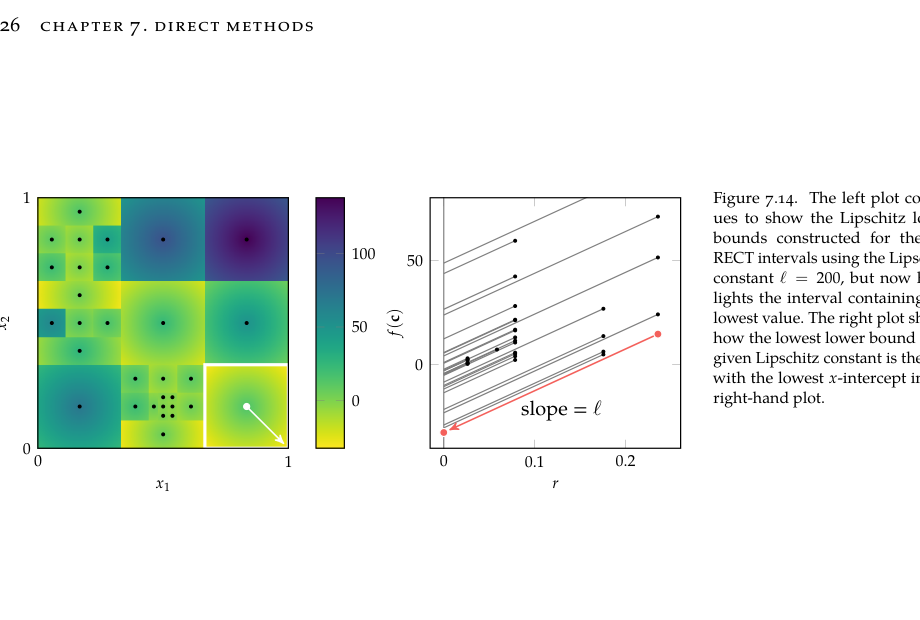
\includegraphics[width=\linewidth]{book_cem_fig.png}
\column{0.45\textwidth}
{\small CEM applied to a 1D function (shown as a blue curve). The Gaussian proposal distribution (shaded region) starts broad and gradually narrows onto the global minimum over successive iterations.}
\end{columns}

\framebreak

\begin{exampleblock}{Worked Example: CEM on the Branin Function (Example 8.3)}
The Branin function is a 2D test function with three global minima all achieving $f^* \approx 0.398$.
Starting from $\bm{\mu}_0 = (0.5, 5.0)$ with $\bm{\Sigma}_0 = \mathbf{I}$ (the identity matrix), using $m = 40$ samples per iteration and $m_\text{elite} = 10$ elite samples:

\begin{center}
\begin{tabular}{rccr}
\toprule
Iteration & $\mu_1$ & $\mu_2$ & $f(\bm{\mu})$ \\
\midrule
0    & 0.50  & 5.00  & 51.8 \\
2    & $-0.12$ & 4.21  & 12.3 \\
4    & $-2.1$  & 12.1  &  3.4 \\
6    & $-3.1$  & 12.3  &  0.9 \\
8    & $-3.14$ & 12.27 &  0.40 \\
10   & $-3.14$ & 12.27 &  0.398 \\
\bottomrule
\end{tabular}
\end{center}
In just 10 iterations (400 total function evaluations), the algorithm converges to the global minimum from a starting point with $f = 51.8$ --- a reduction of more than 99\%.
\end{exampleblock}

\begin{block}{Choosing the Elite Fraction}
The ratio $m_\text{elite}/m$ is a critical hyperparameter:
\begin{itemize}
  \item If $m_\text{elite}/m \to 1$: the refitted distribution closely matches the current proposal, meaning the update is very small and convergence is very slow.
  \item If $m_\text{elite}/m \to 0$: only a tiny number of samples drive the update, making it highly noisy and potentially unstable.
  \item Typical choice: $m_\text{elite} \approx m/10$. This provides a stable but responsive update.
\end{itemize}
\end{block}

\begin{center}
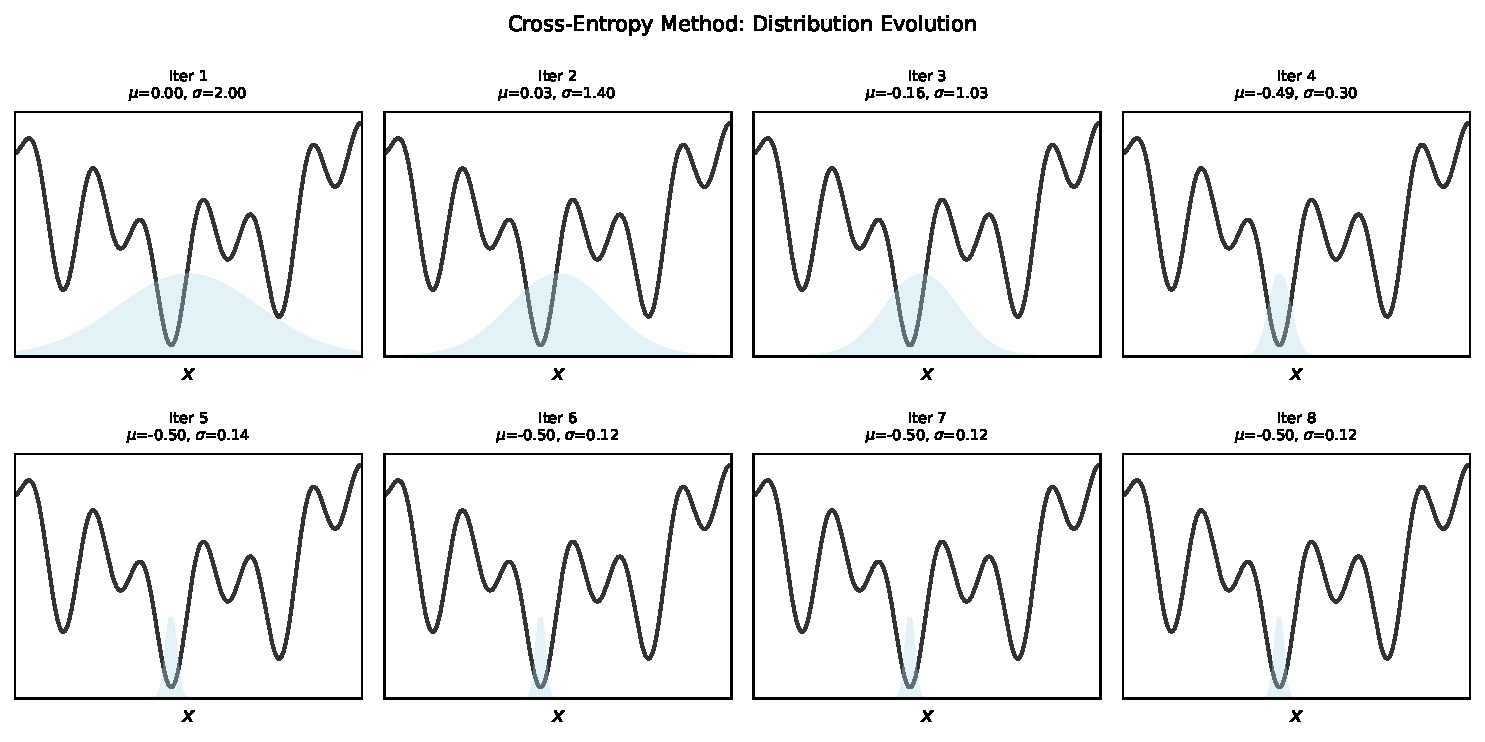
\includegraphics[width=0.55\linewidth]{cem_evolution.pdf}
\end{center}
{\small CEM applied to a 1D multi-modal function. The Gaussian proposal (blue shading) narrows onto the global minimum over iterations, ignoring the local minima.}

\end{frame}

\begin{frame}[fragile]{8.5 Cross-Entropy Method --- Python Implementation}
\begin{lstlisting}[caption={Cross-entropy method with Gaussian proposal (Algorithm 8.8)}]
import numpy as np

def cross_entropy_method(f, mu0, Sigma0, k_max=50, m=100, m_elite=10):
    """
    f       : objective to MINIMISE  R^n -> R
    mu0     : initial mean  (n,)
    Sigma0  : initial covariance  (n,n)
    m       : total samples per iteration
    m_elite : number of elite samples used for refitting
    Returns : estimated minimiser (final mean)
    """
    mu    = np.array(mu0, dtype=float)
    Sigma = np.array(Sigma0, dtype=float)

    for k in range(k_max):
        # Sample from proposal distribution
        samples = np.random.multivariate_normal(mu, Sigma, m)  # (m, n)
        values  = np.array([f(x) for x in samples])

        # Select elite samples (lowest f values)
        elite_idx = np.argsort(values)[:m_elite]
        elite     = samples[elite_idx]

        # Refit distribution (MLE for multivariate Gaussian)
        mu    = elite.mean(axis=0)
        diff  = elite - mu
        Sigma = (diff.T @ diff) / m_elite + np.eye(len(mu)) * 1e-6

    return mu

# Minimise Branin function (2D, 3 global minima)
def branin(x):
    x1, x2 = x[0], x[1]
    a,b,c  = 1, 5.1/(4*np.pi**2), 5/np.pi
    r,s,t  = 6, 10, 1/(8*np.pi)
    return a*(x2 - b*x1**2 + c*x1 - r)**2 + s*(1-t)*np.cos(x1) + s

mu0    = np.array([0.5, 5.0])
Sigma0 = np.array([[1.0, 0.2], [0.2, 1.0]])
x_opt  = cross_entropy_method(branin, mu0, Sigma0)
print(f"CEM solution: {x_opt}, f = {branin(x_opt):.4f}")
\end{lstlisting}
\end{frame}

%%=============================================================================
\section{8.6 Proposal Distribution Descent}
%%=============================================================================

\begin{frame}[allowframebreaks]{8.6 Proposal Distribution Descent (PDD)}

The Cross-Entropy Method updates the proposal distribution by fitting it to elite samples --- a heuristic procedure.
Proposal Distribution Descent (PDD) takes a more principled approach: it directly differentiates the \emph{expected objective} with respect to the distribution parameters $\bm{\theta}$ (bold theta), and performs gradient descent on those parameters.

The goal is to minimise the expected value of $f$ under the proposal distribution:
\[
  J(\bm{\theta}) \;=\; \mathbb{E}_{\mathbf{x} \sim p_\theta}\!\left[f(\mathbf{x})\right]
\]

\begin{block}{Notation for the Expected Objective}
\begin{itemize}
  \item $J(\bm{\theta})$ (J of theta) is the objective we want to minimise --- the average of $f(\mathbf{x})$ when $\mathbf{x}$ is drawn randomly from our proposal distribution $p_\theta$.
  \item $\bm{\theta}$ (bold theta) are the parameters of the proposal distribution. For a Gaussian, $\bm{\theta} = (\mu, \nu)$ where $\mu$ (mu) is the mean and $\nu$ (nu) is the variance.
  \item $\mathbb{E}_{\mathbf{x} \sim p_\theta}[\cdot]$ (E subscript x tilde p-theta) means ``expected value when $\mathbf{x}$ is sampled from $p_\theta$''.
\end{itemize}
\end{block}

\begin{block}{Score Function Gradient (the REINFORCE Trick)}
Computing $\nabla_\theta J$ is non-trivial because the distribution $p_\theta$ itself depends on $\theta$. The score function estimator (also known as the REINFORCE trick) gives:
\[
  \nabla_\theta J(\bm{\theta}) \;=\; \mathbb{E}_{\mathbf{x} \sim p_\theta}\!\left[f(\mathbf{x})\,\nabla_\theta \log p_\theta(\mathbf{x})\right]
\]
The term $\nabla_\theta \log p_\theta(\mathbf{x})$ (nabla-theta of log p-theta of x) is called the \emph{score function}. It measures how much the log-probability of observing $\mathbf{x}$ changes when we tweak the distribution parameters $\bm{\theta}$.

This expectation can be estimated by a Monte Carlo average over $m$ samples:
\[
  \nabla_\theta J \;\approx\; \frac{1}{m}\sum_{i=1}^{m} f\!\left(\mathbf{x}^{(i)}\right)\,\nabla_\theta \log p_\theta\!\left(\mathbf{x}^{(i)}\right)
\]
where each $\mathbf{x}^{(i)} \sim p_\theta$. This is an unbiased estimator of the true gradient.
\end{block}

\begin{block}{Explicit Score Functions for a 1D Gaussian $\mathcal{N}(\mu, \nu)$}
For a one-dimensional Gaussian distribution with mean $\mu$ (mu) and variance $\nu$ (nu), the score functions with respect to each parameter are:
\[
  \nabla_\mu \log \mathcal{N}(x;\mu,\nu) \;=\; \frac{x - \mu}{\nu}
  \qquad \text{and} \qquad
  \nabla_\nu \log \mathcal{N}(x;\mu,\nu) \;=\; \frac{(x-\mu)^2 - \nu}{2\nu^2}
\]
These tell us: if we see a sample $x$ that is larger than $\mu$, the score with respect to $\mu$ is positive, meaning increasing $\mu$ increases the probability of observing $x$. Similarly, a sample with a squared deviation $(x-\mu)^2$ larger than $\nu$ indicates the distribution is too narrow.
\end{block}

\begin{alertblock}{Important Numerical Issue: Variance Can Go Negative}
When the mean $\mu$ is near the optimum $x^*$, the gradient with respect to $\nu$ (nu, the variance) is \emph{positive}. Gradient descent on $\nu$ therefore \emph{decreases} $\nu$ toward zero. As $\nu \to 0$, the term $1/(2\nu^2)$ in the score function grows without bound, making the gradient estimate very large and noisy. With any fixed step size $\alpha$, the update $\nu \leftarrow \nu - \alpha \nabla_\nu J$ will eventually drive $\nu$ to a negative value --- which is invalid since a variance must be positive.

The fix is to reparameterise: let $\nu = e^\eta$ (e to the power eta), so that $\nu$ is always positive regardless of the value of $\eta$ (eta). We then perform gradient descent on $\eta$ instead.
\end{alertblock}

\begin{columns}[T]
\column{0.52\textwidth}
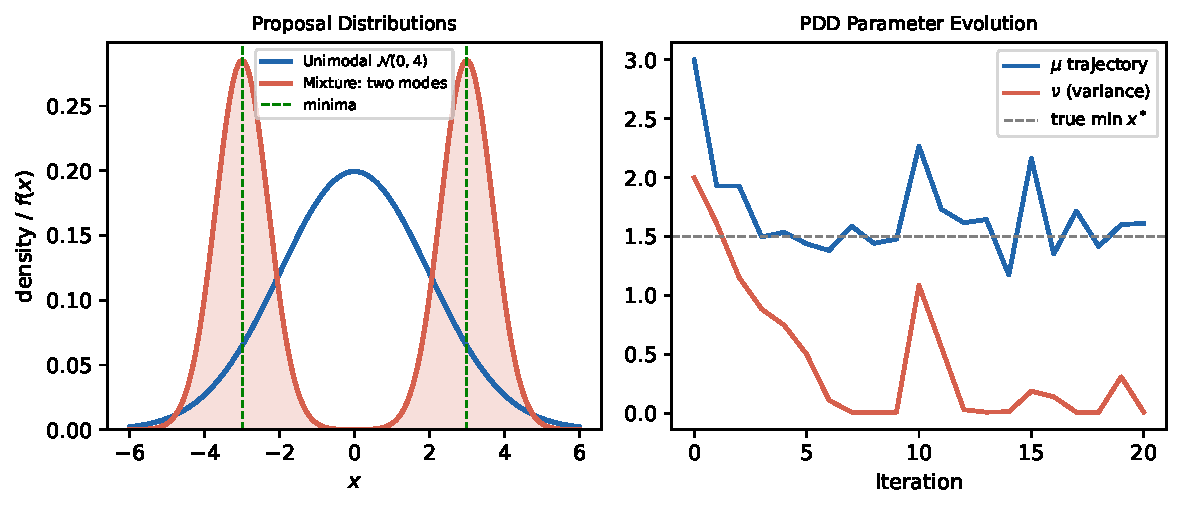
\includegraphics[width=\linewidth]{pdd_illustration.pdf}
\column{0.45\textwidth}
{\small \textbf{Left:} A unimodal Gaussian proposal concentrates on a single mode, while a mixture proposal can capture multiple modes simultaneously. \textbf{Right:} PDD parameter evolution ($\mu$ and $\nu$) on a noisy multi-modal objective over iterations.}
\end{columns}

\end{frame}

\begin{frame}[fragile]{8.6 PDD --- Python Implementation}
\begin{lstlisting}[caption={Proposal distribution descent with Gaussian proposal (Algorithm 8.9)}]
import numpy as np

def proposal_distribution_descent(f, mu0, nu0, alpha=0.1, m=50, n_iter=200):
    """
    Minimise E_{x~N(mu,nu)}[f(x)] via score-function gradient.
    f    : objective R -> R
    mu0  : initial mean
    nu0  : initial variance (>0)
    """
    mu, log_nu = float(mu0), np.log(float(nu0))  # nu = exp(log_nu) > 0

    for _ in range(n_iter):
        nu = np.exp(log_nu)
        xs = np.random.normal(mu, np.sqrt(nu), m)
        fs = np.array([f(x) for x in xs])

        # Score-function gradients
        score_mu = (xs - mu) / nu
        score_nu = ((xs - mu)**2 - nu) / (2 * nu**2)

        g_mu     = np.mean(fs * score_mu)
        g_nu     = np.mean(fs * score_nu)

        # Update (reparameterise nu = exp(log_nu) to keep nu > 0)
        g_log_nu = g_nu * nu             # chain rule
        mu     -= alpha * g_mu
        log_nu -= alpha * g_log_nu

    return mu, np.exp(log_nu)

# Multi-modal target: minimize f = sin(3x)*cos(x) + 0.05*x^2
f_mm = lambda x: np.sin(3*x)*np.cos(x) + 0.05*x**2
mu_opt, nu_opt = proposal_distribution_descent(f_mm, mu0=0.5, nu0=4.0)
print(f"PDD: mu*={mu_opt:.3f}, nu*={nu_opt:.4f}, f={f_mm(mu_opt):.4f}")
\end{lstlisting}
\end{frame}

%%=============================================================================
\section{8.7 Information-Geometric Optimization (IGO)}
%%=============================================================================

\begin{frame}[allowframebreaks]{8.7 Information-Geometric Optimization (IGO)}

PDD performs gradient descent in the space of distribution parameters $\bm{\theta}$.
However, this ordinary gradient is sensitive to how we parameterise the distribution: a different but equivalent parameterisation (e.g., using the precision $1/\nu$ instead of the variance $\nu$) gives a different gradient and a different optimisation trajectory.
This lack of \emph{invariance} is a practical problem: the algorithm's behaviour depends on an arbitrary modelling choice.

Information-Geometric Optimization (IGO) fixes this by using the \emph{natural gradient} instead of the ordinary gradient.
The natural gradient accounts for the intrinsic geometry of the space of probability distributions, making the update invariant to reparameterisation.

\begin{block}{The Fisher Information Matrix}
The Fisher information matrix $\mathbf{F}(\bm{\theta})$ (bold F of theta) measures how much information a single observation from $p_\theta$ carries about the parameters $\bm{\theta}$:
\[
  \mathbf{F}(\bm{\theta}) \;=\; \mathbb{E}_{\mathbf{x} \sim p_\theta}\!\left[\nabla_\theta \log p_\theta(\mathbf{x})\,\left(\nabla_\theta \log p_\theta(\mathbf{x})\right)^\top\right]
\]
This is a square matrix of size (number of parameters) $\times$ (number of parameters). It acts as a local ``metric tensor'' on the space of distributions --- it measures how different two nearby distributions are in terms of the information they carry.
\end{block}

\begin{block}{The Natural Gradient Update}
The natural gradient $\tilde{\nabla}_\theta J$ is obtained by pre-multiplying the ordinary gradient by the inverse Fisher information matrix:
\[
  \tilde{\nabla}_\theta J \;=\; \mathbf{F}^{-1}(\bm{\theta})\,\nabla_\theta J(\bm{\theta})
\]
The IGO update is then:
\[
  \bm{\theta}^{(k+1)} \;\leftarrow\; \bm{\theta}^{(k)} - \alpha\,\tilde{\nabla}_\theta J(\bm{\theta}^{(k)})
\]
Pre-multiplying by $\mathbf{F}^{-1}$ (F inverse) ``stretches'' or ``squashes'' the gradient vector to correct for the curvature of the distribution manifold, just as one would correct for the curvature of a physical surface when computing shortest paths.
\end{block}

\begin{alertblock}{How to Read the Natural Gradient}
Think of the parameter space as a curved surface (a Riemannian manifold). In flat Euclidean space, the steepest descent direction is simply $-\nabla J$. On a curved surface, the steepest descent must account for the surface's curvature --- otherwise a step that looks large in parameter space may correspond to a tiny change in the actual distribution. The Fisher matrix $\mathbf{F}$ encodes this curvature, and $\mathbf{F}^{-1} \nabla J$ is the correctly scaled steepest descent direction on the curved surface.
\end{alertblock}

\begin{block}{Natural Gradient for a Multivariate Gaussian $\mathcal{N}(\bm{\mu}, \bm{\Sigma})$}
For a Gaussian proposal, the natural gradient updates simplify to remarkably clean formulas (equations 8.25--8.26 in the textbook):
\[
  \tilde{\nabla}_{\mu} J \;=\; \mathbb{E}\!\left[f(\mathbf{x})\,(\mathbf{x} - \bm{\mu})\right]
\]
\[
  \tilde{\nabla}_{\Sigma} J \;=\; \frac{1}{2}\,\mathbb{E}\!\left[f(\mathbf{x})\!\left((\mathbf{x}-\bm{\mu})(\mathbf{x}-\bm{\mu})^\top - \bm{\Sigma}\right)\right]
\]
These are estimated by Monte Carlo averaging over samples.
\end{block}

\begin{block}{Why IGO Uses Fitness Rankings, Not Raw Values}
A key property of IGO is that the update is invariant to any \emph{order-preserving transformation} of $f$: replacing $f(\mathbf{x})$ with $g(f(\mathbf{x}))$ for any increasing function $g$ produces the same distribution trajectory.
In practice, this is implemented by replacing raw $f$ values with \emph{rank-based weights}: the best sample gets weight $w_1$, the second-best gets $w_2$, etc.
This makes IGO robust to outliers and eliminates the need to tune the absolute scale of $f$.
\end{block}

\begin{columns}[T]
\column{0.55\textwidth}
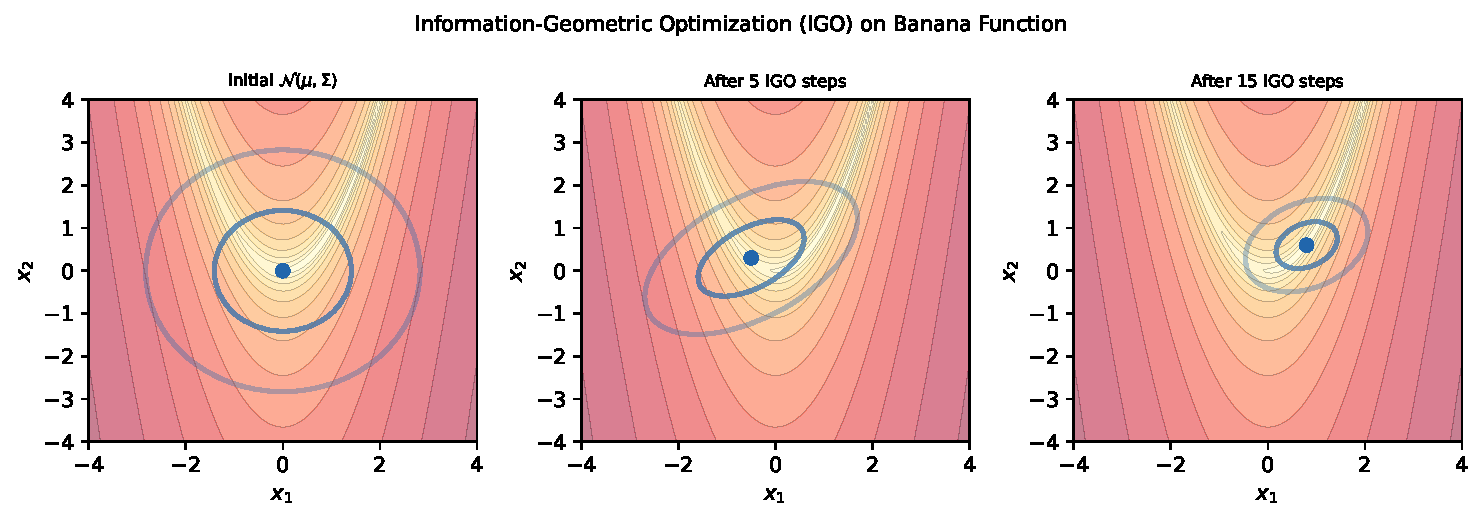
\includegraphics[width=\linewidth]{igo_illustration.pdf}
\column{0.42\textwidth}
{\small IGO distributions converging on the Banana (Rosenbrock) function, a notoriously difficult test problem with a curved, narrow valley. The ellipses show the 1-sigma contours of the Gaussian proposal at successive iterations. Fisher information removes scale dependence, allowing the ellipse to align with the valley.}
\end{columns}

\end{frame}

\begin{frame}[fragile]{8.7 IGO --- Python Implementation (Algorithm 8.10)}
\begin{lstlisting}[caption={Information-geometric optimisation with multivariate Gaussian}]
import numpy as np

def information_geometric_optimization(f, mu0, Sigma0, k_max=100, alpha=1.0):
    """
    Algorithm 8.10: IGO with multivariate normal.
    Sample size m = 4 + floor(3*log(n)).
    Elite fraction: half the samples (ranked weighting).
    """
    mu    = np.array(mu0, dtype=float)
    Sigma = np.array(Sigma0, dtype=float)
    n     = len(mu)

    m        = 4 + int(3 * np.log(n))         # population size
    m_elite  = m // 2                          # number of elite samples

    # Log-based weights (eq. 8.29): rank 1 = best
    ws = np.log(m_elite + 1) - np.log(np.arange(1, m_elite + 1))
    ws /= ws.sum()                             # normalise to sum to 1

    for _ in range(k_max):
        # Sample and evaluate
        xs = np.random.multivariate_normal(mu, Sigma, m)
        ys = np.array([f(x) for x in xs])
        order = np.argsort(ys)                 # best to worst

        # Weighted natural gradient updates
        delta_mu    = np.zeros(n)
        delta_Sigma = np.zeros((n, n))
        for i, wi in zip(order[:m_elite], ws):
            d = xs[i] - mu
            delta_mu    += wi * d
            delta_Sigma += wi * (np.outer(d, d) - Sigma)

        mu    += alpha * delta_mu
        Sigma += alpha * delta_Sigma
        Sigma  = (Sigma + Sigma.T) / 2        # enforce symmetry

    return mu, Sigma

f_rosen = lambda x: (1-x[0])**2 + 100*(x[1]-x[0]**2)**2
mu_opt, S_opt = information_geometric_optimization(
    f_rosen, [0.,0.], np.eye(2)*2, k_max=200)
print(f"IGO: mu*={mu_opt}, f={f_rosen(mu_opt):.6f}")  # near [1,1]
\end{lstlisting}
\end{frame}

%%=============================================================================
\section{8.8 Covariance Matrix Adaptation (CMA-ES)}
%%=============================================================================

\begin{frame}[allowframebreaks]{8.8 Covariance Matrix Adaptation Evolution Strategy (CMA-ES)}

CMA-ES (Hansen \& Ostermeier, 2001) extends IGO by making a critical distinction: it separates the \emph{overall scale} of the search (controlled by a scalar step size $\sigma$ (sigma)) from the \emph{shape and orientation} of the search (controlled by a shape matrix $\mathbf{C}$ (bold C)).

This separation allows CMA-ES to independently adapt how large to search (expanding when progress is fast, contracting when it stalls) and which directions to search preferentially (rotating and stretching the search ellipsoid to align with the problem's natural axes).

\begin{block}{The CMA-ES Sampling Distribution}
At each iteration, candidate solutions are drawn from:
\[
  \mathbf{x}^{(i)} \;\sim\; \mathcal{N}\!\left(\bm{\mu},\; \sigma^2 \mathbf{C}\right)
\]
where:
\begin{itemize}
  \item $\bm{\mu}$ (bold mu) is the current mean of the distribution --- the algorithm's best estimate of the location of the minimum.
  \item $\sigma$ (sigma) is the global step size --- a positive scalar controlling the overall scale of the search. Adapting $\sigma$ is analogous to adapting the learning rate in SGD.
  \item $\mathbf{C}$ (bold C) is the shape matrix (a covariance matrix normalised so that its determinant is 1). It encodes the preferred search directions. When $\mathbf{C} = \mathbf{I}$ (the identity matrix), search is isotropic (equal in all directions). When $\mathbf{C}$ is elongated, search is preferentially in the elongated direction.
\end{itemize}
\end{block}

\begin{block}{The Mean Update (Same as IGO)}
\[
  \bm{\mu}' \;=\; \bm{\mu} \;+\; \alpha_\mu \sum_{i=1}^{m} w_i\!\left(\mathbf{x}^{[i]} - \bm{\mu}\right)
\]
Here $[i]$ (brackets around $i$) means the $i$-th best sample (rank 1 = best), $w_i$ (w sub i) are positive weights that sum to 1, and $\alpha_\mu$ (alpha sub mu) is a step size for the mean update (typically 1). This is a weighted average update: the mean moves toward the weighted centroid of the elite samples.
\end{block}

\begin{block}{Evolution Paths: Accumulating Direction Information}
CMA-ES introduces two ``evolution paths'' --- running averages of the steps taken by the mean over recent iterations. These paths accumulate information about the direction and speed of progress.

The \textbf{sigma-path} $\mathbf{p}_\sigma$ (p sub sigma) tracks the cumulated step direction for step-size control:
\[
  \mathbf{p}_\sigma^{(k+1)} \;=\; (1-\alpha_\sigma)\mathbf{p}_\sigma^{(k)}
    \;+\; \sqrt{\alpha_\sigma(2-\alpha_\sigma)m_\text{eff}}\;\frac{\bm{\mu}'-\bm{\mu}}{\sigma}
\]

The \textbf{C-path} $\mathbf{p}_c$ (p sub c) tracks the cumulated step direction for covariance adaptation:
\[
  \mathbf{p}_c^{(k+1)} \;=\; (1-\alpha_c)\mathbf{p}_c^{(k)}
    \;+\; \sqrt{\alpha_c(2-\alpha_c)m_\text{eff}}\;\frac{\bm{\mu}'-\bm{\mu}}{\sigma}
\]
\end{block}

\begin{block}{Notation for the Evolution Paths}
\begin{itemize}
  \item $\alpha_\sigma$ (alpha sub sigma) and $\alpha_c$ (alpha sub c) are decay constants in $(0,1)$ controlling how quickly old information is forgotten. Typical values are around $1/\sqrt{n}$.
  \item $(1-\alpha_\sigma)\mathbf{p}_\sigma^{(k)}$ is the ``faded'' old path --- old information is down-weighted exponentially.
  \item The second term adds the current normalised step $(\bm{\mu}' - \bm{\mu})/\sigma$, scaled by $\sqrt{\alpha_\sigma(2-\alpha_\sigma)m_\text{eff}}$ to keep the path length statistically calibrated.
  \item $m_\text{eff}$ (m sub eff) is the effective population size: $m_\text{eff} = 1/\sum_i w_i^2$. It measures how many samples are contributing effectively to the update. A high $m_\text{eff}$ means the weights are spread evenly; a low $m_\text{eff}$ means one or two samples dominate.
\end{itemize}
\end{block}

\begin{alertblock}{Why Evolution Paths Are Powerful}
Without evolution paths, the covariance update would only use information from the current iteration's samples --- a very noisy signal. By accumulating the direction of movement across many iterations, the evolution path provides a much cleaner signal. If the algorithm consistently moves in the same direction over multiple iterations, the evolution path becomes long and the algorithm learns to preferentially search in that direction.
\end{alertblock}

\framebreak

\begin{block}{Step-Size Control}
The global step size $\sigma$ is updated based on the length of the sigma-path:
\[
  \sigma^{(k+1)} \;=\; \sigma^{(k)} \exp\!\left(\frac{\alpha_\sigma}{\beta_\sigma}\left(
    \frac{\|\mathbf{p}_\sigma\|}{\mathbb{E}[\|\mathcal{N}(\mathbf{0},\mathbf{I})\|]} - 1\right)\right)
\]
\end{block}

\begin{block}{Notation for Step-Size Control}
\begin{itemize}
  \item $\|\mathbf{p}_\sigma\|$ (the norm, or length, of the sigma-path) is compared to $\mathbb{E}[\|\mathcal{N}(\mathbf{0},\mathbf{I})\|]$, the expected length of a standard Gaussian random vector. This expected length is $\sqrt{2}\,\Gamma((n+1)/2)/\Gamma(n/2)$ where $\Gamma$ (Gamma) is the Gamma function (a generalisation of the factorial).
  \item If $\|\mathbf{p}_\sigma\|$ is \emph{larger} than expected, the algorithm has been consistently moving in the same direction --- a sign that the step size should be \emph{increased} to make faster progress.
  \item If $\|\mathbf{p}_\sigma\|$ is \emph{smaller} than expected, the algorithm has been oscillating, changing direction frequently --- a sign that the step size should be \emph{decreased} to improve accuracy.
  \item $\beta_\sigma$ (beta sub sigma) is a damping coefficient (typically 1.0) that prevents the step size from changing too rapidly.
\end{itemize}
\end{block}

\begin{block}{Covariance Matrix Update}
The shape matrix $\mathbf{C}$ is updated using a combination of a rank-1 update (from the C-path) and a rank-$m$ update (from the current elite samples):
\[
  \mathbf{C}^{(k+1)} \;=\; (1-\alpha_1-\alpha_e)\mathbf{C}^{(k)}
  \;+\; \alpha_1 \mathbf{p}_c \mathbf{p}_c^\top
  \;+\; \frac{\alpha_e}{\sigma^2}\sum_{i=1}^{m} w_i \mathbf{x}^{[i]}(\mathbf{x}^{[i]})^\top
\]
\begin{itemize}
  \item The \textbf{rank-1 update} ($\alpha_1 \mathbf{p}_c \mathbf{p}_c^\top$) stretches the covariance in the direction of the evolution path, exploiting correlated steps accumulated over time. Here $\alpha_1$ (alpha sub 1) controls the learning rate of this term.
  \item The \textbf{rank-$m$ update} (the sum over elite samples) uses the current generation's best samples to update the covariance, exploiting correlations within a single iteration. Here $\alpha_e$ (alpha sub e) is the corresponding learning rate.
\end{itemize}
\end{block}

\begin{block}{Default Hyperparameters for an $n$-Dimensional Problem}
\begin{center}
\begin{tabular}{ll}
\toprule
Parameter & Value \\
\midrule
Population size $m$ & $4 + \lfloor 3 \ln n \rfloor$ \\
Elite size $m_e$ & $m / 2$ (rounded down) \\
Rank-1 learning rate $\alpha_1$ & $2 / n^2$ \\
Rank-$m$ learning rate $\alpha_e$ & $m_e / n^2$ \\
C-path decay $\alpha_c$ & $1/\sqrt{n}$ \\
$\sigma$-path decay $\alpha_\sigma$ & $1/\sqrt{n}$ \\
Damping $\beta_\sigma$ & $1.0$ \\
\bottomrule
\end{tabular}
\end{center}
These defaults are carefully derived from the statistical properties of the algorithm and work well across a wide range of problems without tuning.
\end{block}

\end{frame}

\begin{frame}[fragile]{8.8 CMA-ES --- Python Implementation (Algorithm 8.11)}
\begin{lstlisting}[caption={CMA-ES: covariance matrix adaptation evolution strategy}]
import numpy as np
from scipy.special import gamma as gamma_fn

def cmaes(f, mu0, sigma0=1.0, C0=None, k_max=500):
    n   = len(mu0)
    mu  = np.array(mu0, dtype=float)
    sig = float(sigma0)
    C   = np.eye(n) if C0 is None else np.array(C0, dtype=float)

    m        = 4 + int(3 * np.log(n))
    m_elite  = m // 2
    a1       = 2 / n**2;           ae = m_elite / n**2
    ac       = 1 / np.sqrt(n);     ao = 1 / np.sqrt(n)
    amu      = 1 - a1 - ae;        bs = 1.0
    ws = np.log(m_elite+1) - np.log(np.arange(1, m_elite+1))
    ws /= ws.sum()
    m_eff    = 1 / np.sum(ws**2)
    exp_len  = (np.sqrt(2) * gamma_fn((n+1)/2) / gamma_fn(n/2))
    p_sig = np.zeros(n);           p_c = np.zeros(n)

    for _ in range(k_max):
        xs = np.random.multivariate_normal(mu, sig**2 * C, m)
        ys = np.array([f(x) for x in xs])
        idx = np.argsort(ys)                   # best first

        mu_new = mu + amu * sum(ws[i]*(xs[idx[i]]-mu) for i in range(m_elite))
        delta  = (mu_new - mu) / sig

        # Evolution path updates
        p_sig = (1-ao)*p_sig + np.sqrt(ao*(2-ao)*m_eff)*delta
        p_c   = (1-ac)*p_c   + np.sqrt(ac*(2-ac)*m_eff)*delta

        # Step-size control
        sig  *= np.exp(ao/bs * (np.linalg.norm(p_sig)/exp_len - 1))

        # Covariance update (rank-1 + rank-m)
        C = (amu*C + a1*np.outer(p_c,p_c)
             + ae/sig**2 * sum(ws[i]*np.outer(xs[idx[i]]-mu,
                                              xs[idx[i]]-mu)
                               for i in range(m_elite)))
        C = (C + C.T) / 2           # enforce symmetry
        mu = mu_new
    return mu, sig, C

mu_opt,_,_ = cmaes(lambda x: sum((x-1)**2), [5.]*4, sigma0=2.0)
print(f"CMA-ES: {mu_opt}")   # -> [1, 1, 1, 1]
\end{lstlisting}
\end{frame}

\begin{frame}[allowframebreaks]{8.8 CMA-ES --- Flower Function Example}

\begin{columns}[T]
\column{0.46\textwidth}
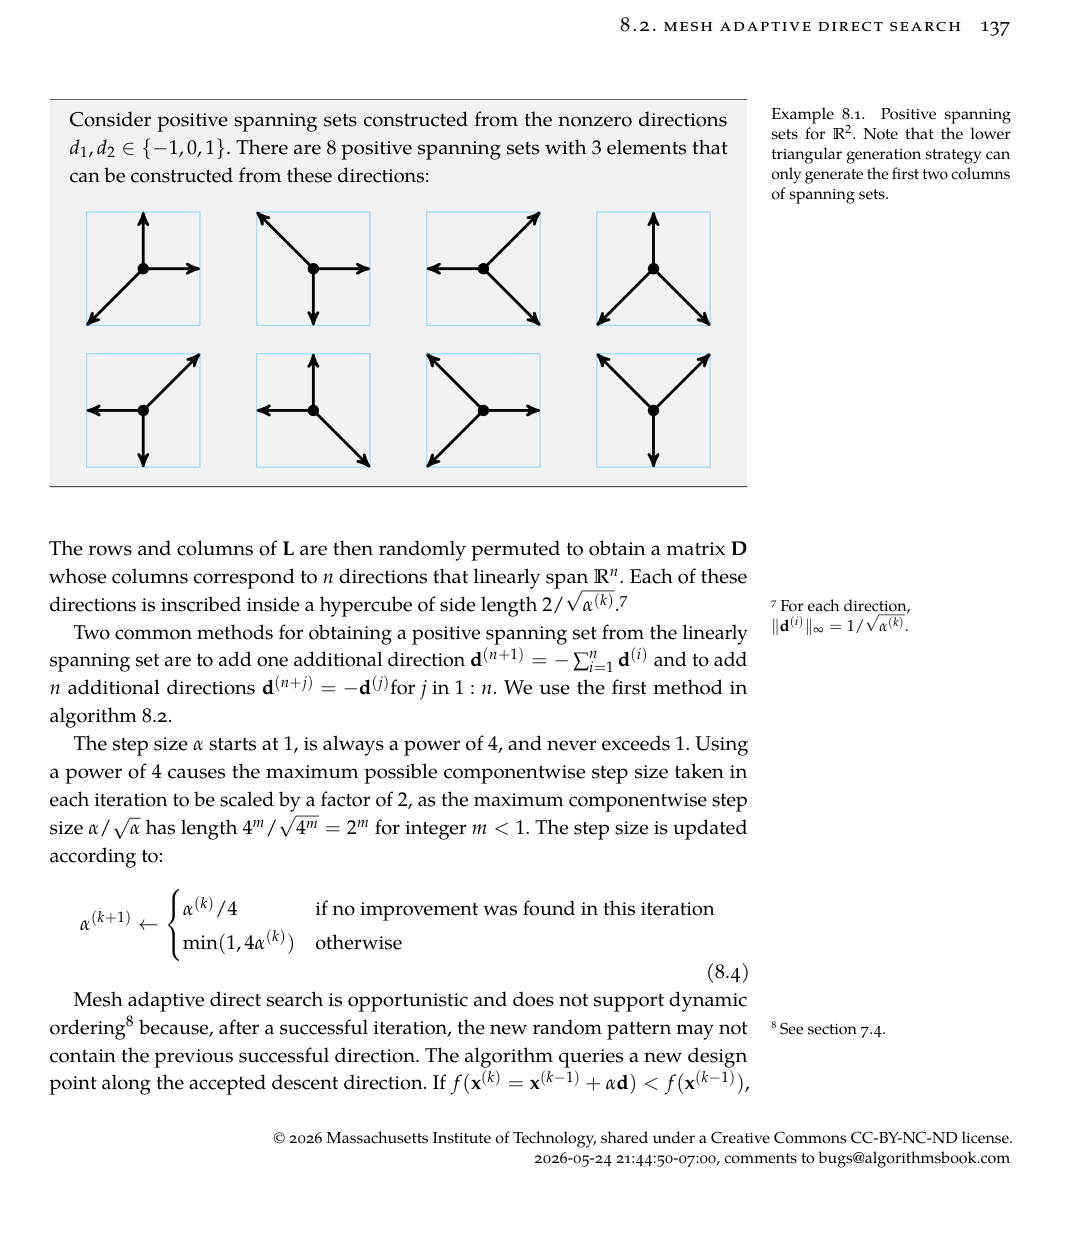
\includegraphics[width=\linewidth]{book_cmaes_flower.png}
\column{0.51\textwidth}
{\small CMA-ES applied to the flower function (a challenging 2D test function with rotational structure, defined in Appendix B.4 of the textbook). Each row shows the distribution's mean and covariance ellipse (the 1-$\sigma$ contour of $\mathcal{N}(\bm{\mu}, \sigma^2\mathbf{C})$) overlaid on the objective's contour plot. Columns correspond to iterations 0, 5, 15, and 40.}
\end{columns}

\begin{block}{What the Flower Example Shows}
\begin{itemize}
  \item \textbf{Iteration 0:} The distribution starts as a large circle (isotropic, $\mathbf{C} = \mathbf{I}$). It covers a broad region of the design space and has no preferred direction.

  \item \textbf{Iteration 5:} The ellipse has begun to rotate and elongate, aligning with the principal curvature direction of the objective function. The algorithm has learned from the first few generations that progress is easier in one direction than the other.

  \item \textbf{Iteration 15:} The covariance has shrunk substantially. The distribution is concentrated in a narrow elliptical region near the minimum, tightly tracking the curved valley of the flower function.

  \item \textbf{Iteration 40:} The distribution has converged: the ellipse is very small, centred near the global minimum, and oriented to match the local geometry of the objective.
\end{itemize}
\end{block}

\begin{block}{Invariance Properties of CMA-ES}
CMA-ES is invariant to three important classes of transformations, which make it robust in practice:
\begin{enumerate}
  \item \textbf{Order-preserving transformations of $f$:} Replacing $f(\mathbf{x})$ with $g(f(\mathbf{x}))$ for any strictly increasing function $g$ (e.g., taking the square root or the logarithm of $f$) does not change the algorithm's trajectory, because CMA-ES uses rank-based weights rather than raw function values.

  \item \textbf{Rotation of the search space:} Rotating all coordinates by any orthogonal matrix does not affect performance, because $\mathbf{C}$ can adapt to any orientation.

  \item \textbf{Scaling of individual coordinates:} Multiplying any coordinate by a constant does not affect performance (up to the time needed for $\mathbf{C}$ and $\sigma$ to adapt).
\end{enumerate}
These properties make CMA-ES particularly effective on ill-conditioned problems, where the objective varies at very different rates in different directions.
\end{block}

\begin{block}{Computational Complexity}
\begin{itemize}
  \item \textbf{Per iteration:} $O(n^2)$ for the covariance update (computing outer products and matrix sums).
  \item \textbf{Eigendecomposition:} Required every $O(n)$ iterations to sample from $\mathcal{N}(\bm{\mu}, \sigma^2\mathbf{C})$ efficiently; costs $O(n^3)$ but is amortised to $O(n^2)$ per iteration.
  \item \textbf{Recommended problem size:} $n$ up to a few hundred. For $n > 1000$, specialised variants (e.g., sep-CMA-ES, which restricts $\mathbf{C}$ to be diagonal) are used.
\end{itemize}
\end{block}

\end{frame}

%%=============================================================================
\section{Method Comparison}
%%=============================================================================

\begin{frame}[allowframebreaks]{Comparing Stochastic Methods}

Having studied eight different stochastic optimisation methods, it is useful to compare them across the dimensions most relevant to practical selection: the order of information used (zeroth vs.\ first), memory requirements, and whether global convergence is guaranteed.

\begin{block}{Summary Comparison Table}
\begin{center}
{\footnotesize
\begin{tabular}{lcccl}
\toprule
Method & Order & Memory & Global convergence? & Best suited for \\
\midrule
Noisy Descent  & 1st & $O(n)$   & No  & Differentiable, large $n$, mini-batch \\
MADS           & 0th & $O(n^2)$ & Asymptotic & Black-box, small $n$, noisy $f$ \\
MeZO           & 0th & $O(1)$   & No  & Huge $n$ (LLMs), memory-limited \\
Sim.\ Annealing & 0th & $O(1)$   & Asymptotic & Discrete/combinatorial, small $n$ \\
Cross-Entropy  & 0th & $O(n^2)$ & Yes (empirically) & Multi-modal, $n < 100$ \\
PDD            & 0th & $O(n^2)$ & No  & Differentiable proposal, $n < 50$ \\
IGO            & 0th & $O(n^2)$ & Yes (invariant) & $n = 10$--$100$, ill-conditioned \\
CMA-ES         & 0th & $O(n^2)$ & Yes (invariant) & $n = 10$--$100$, state of the art \\
\bottomrule
\end{tabular}
}
\end{center}
\end{block}

\begin{block}{Practical Decision Guide}
\begin{itemize}
  \item \textbf{Gradient is available and the model is large ($n > 10{,}000$):} Use noisy descent (SGD) with mini-batches for standard neural networks. Use MeZO if memory is the bottleneck (e.g., fine-tuning LLMs on a single GPU).

  \item \textbf{Black-box objective, small to medium $n$ ($n < 20$):} MADS is a solid first choice --- no gradient needed, provably convergent, and robust to noise. Simulated annealing is competitive when the problem has a combinatorial or discrete structure.

  \item \textbf{Many local minima, $n < 100$:} CMA-ES is generally the state-of-the-art choice. The Cross-Entropy Method is simpler to implement and competitive for moderate $n$.

  \item \textbf{Require theoretical invariance guarantees:} IGO or CMA-ES, which are invariant to reparameterisation and order-preserving transforms of $f$.

  \item \textbf{Very large $n$ ($n > 10^6$), zeroth-order required:} MeZO, which requires only $O(1)$ extra memory regardless of model size.
\end{itemize}
\end{block}

\begin{center}
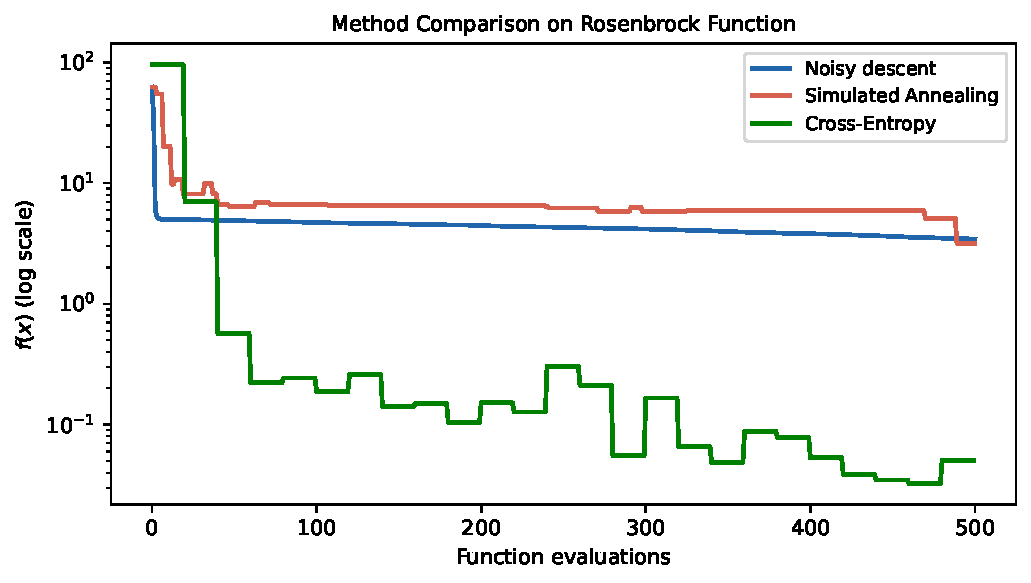
\includegraphics[width=0.60\linewidth]{method_comparison.pdf}
\end{center}
{\small Noisy descent, simulated annealing, and the cross-entropy method applied to the Rosenbrock function starting from $(-1.5, 1.5)$. All three reach the vicinity of the minimum at $(1, 1)$, but CEM converges most directly while SA takes a more wandering path.}

\end{frame}

%%=============================================================================
\section{8.9--8.10 Summary \& Exercises}
%%=============================================================================

\begin{frame}[allowframebreaks]{8.9 Chapter Summary}

This chapter introduced stochastic optimisation methods --- algorithms that deliberately incorporate randomness to escape local minima, handle noisy objectives, and explore large design spaces.
Here is a concise summary of each method covered.

\begin{block}{Noisy Descent (Section 8.1)}
Noisy descent adds Gaussian random noise to the gradient at each step. The key requirement is that the noise be \emph{unbiased} (zero mean), so that the expected update equals the true gradient direction. The Robbins--Monro step-size conditions --- the step sizes must sum to infinity but their squares must sum to a finite value --- guarantee convergence. A classic schedule satisfying these conditions is $\alpha^{(k)} = \alpha^{(1)}/k$.
\end{block}

\begin{block}{Mesh Adaptive Direct Search / MADS (Section 8.2)}
MADS is a pattern-search method requiring only function values. It generates random positive spanning sets of search directions at each iteration using a lower-triangular random matrix, probes the objective in each direction, and updates the step size by a factor of 4 (expanding on success, contracting on failure). Because the step size is always a power of $\tfrac{1}{4}$, the resulting mesh becomes arbitrarily fine, guaranteeing convergence.
\end{block}

\begin{block}{MeZO (Section 8.3)}
MeZO estimates the gradient using only two forward function evaluations and a re-seeded PRNG. No backward pass is needed. By re-generating the random direction $\mathbf{z}$ from the same seed for the parameter update, the method requires $O(1)$ extra memory regardless of the number of parameters --- making it practical for fine-tuning models with billions of parameters.
\end{block}

\begin{block}{Simulated Annealing (Section 8.4)}
Simulated annealing controls exploration via a ``temperature'' parameter $t$ that decreases over time. Proposed moves that \emph{worsen} the objective are accepted with probability $e^{-\Delta y / t}$ --- small for large worsening or low temperature, but substantial for small worsening at high temperature. The Boltzmann cooling schedule $t^{(k)} \propto 1/\ln(k)$ guarantees asymptotic convergence to the global minimum; the faster exponential schedule is more practical. Adaptive SA (Section 8.4) additionally adjusts the step size per coordinate to maintain a 50\% acceptance rate.
\end{block}

\begin{block}{Cross-Entropy Method (Section 8.5)}
CEM maintains a Gaussian proposal distribution over the design space. At each iteration, it samples candidates, selects the best fraction as the elite set, and refits the Gaussian to those elite samples using maximum likelihood estimation (MLE gives the sample mean and covariance). The distribution progressively narrows onto the region of best performance. The elite fraction (typically $m_\text{elite} \approx m/10$) is the most critical hyperparameter.
\end{block}

\begin{block}{Proposal Distribution Descent (Section 8.6)}
PDD directly differentiates the expected objective $J(\bm{\theta}) = \mathbb{E}_{x \sim p_\theta}[f(x)]$ with respect to the distribution parameters $\bm{\theta}$ using the score function (REINFORCE) estimator. Unlike CEM, it does not use elite sample selection. The variance parameter must be reparameterised (e.g., $\nu = e^\eta$) to prevent it from going negative.
\end{block}

\begin{block}{Information-Geometric Optimization (Section 8.7)}
IGO applies the \emph{natural gradient} --- the ordinary gradient pre-multiplied by the inverse Fisher information matrix. This makes the updates invariant to reparameterisation of the distribution and to order-preserving transformations of $f$. In practice, raw function values are replaced by rank-based weights. For a Gaussian proposal, the natural gradient has a particularly clean closed form.
\end{block}

\begin{block}{CMA-ES (Section 8.8)}
CMA-ES extends IGO by separately tracking a global step size $\sigma$ and a shape matrix $\mathbf{C}$. Two ``evolution paths'' --- running averages of recent mean movements --- accumulate directional information across iterations, enabling efficient learning of the covariance structure. Step size is adapted based on whether the evolution path length is consistent with random walk behaviour. CMA-ES is generally considered the state-of-the-art method for zeroth-order optimisation in $n = 10$ to $n = 100$ dimensions.
\end{block}

\end{frame}

\begin{frame}[allowframebreaks]{8.10 Exercises}

\begin{block}{Exercise 8.1: Limitations of Mixture Proposals in CEM}
We have seen that mixture proposal distributions can better capture multiple modes of the objective (e.g., multiple global minima separated in space). Why might their use in the cross-entropy method be limited in practice?

\medskip
\textit{Solution:} The cross-entropy method requires fitting the proposal distribution to the elite samples at every iteration using maximum likelihood estimation (MLE). For a single Gaussian, MLE has an analytic closed form (the sample mean and covariance). Unfortunately, no known analytic solutions exist for fitting multivariate Gaussian \emph{mixture} distributions. The standard alternative is the Expectation--Maximisation (EM) algorithm, which is itself an iterative procedure requiring many iterations to converge at each outer CEM iteration. This nested optimisation is computationally expensive and makes mixture proposals impractical for CEM in most real applications.
\end{block}

\begin{block}{Exercise 8.2: Effect of Elite Fraction in CEM}
In the cross-entropy method, what is the potential effect of using an elite sample size $m_\text{elite}$ that is very close to the total sample size $m$?

\medskip
\textit{Solution:} If $m_\text{elite}/m \to 1$ (elite fraction approaches 100\%), almost all samples are considered ``elite'' regardless of their objective values. The refitted Gaussian will closely match the current proposal distribution, because nearly all samples are used in the MLE update. There is no strong selection pressure toward better regions of the design space, so the mean barely moves and the covariance barely shrinks. The result is extremely slow convergence: the algorithm makes negligible progress per iteration. This is analogous to natural selection with no selection pressure --- all individuals survive equally, so the population does not evolve toward fitter traits.
\end{block}

\framebreak

\begin{block}{Exercise 8.3: Variance Instability in PDD}
Consider proposal distribution descent with $\mathcal{N}(\mu, \nu)$, with the mean sitting at the optimum: $\mu = x^*$.
Show that the gradient of $J$ with respect to $\nu$ (nu, the variance) is positive, which means gradient descent decreases $\nu$ toward zero.
Explain why a fixed step size $\alpha$ (alpha) poses a numerical risk as $\nu \to 0$.

\medskip
\textit{Solution:} Near the optimum, approximate $f(x) \approx \frac{1}{2}h(x-x^*)^2$ where $h = f''(x^*) > 0$ (h is the second derivative, which is positive because $x^*$ is a minimum). Substituting into the expected objective:
\[
  J(\mu, \nu) = \mathbb{E}_{x \sim \mathcal{N}(\mu,\nu)}\!\left[\tfrac{1}{2}h(x-\mu)^2\right] = \tfrac{1}{2}h\nu
\]
Therefore $\nabla_\nu J = \tfrac{1}{2}h > 0$. Gradient descent on $\nu$ applies the update $\nu \leftarrow \nu - \alpha \cdot \tfrac{1}{2}h$, which decreases $\nu$ each iteration. Eventually $\nu$ reaches zero and then goes negative, which is invalid (a variance must be non-negative).

Moreover, as $\nu \to 0$, the score function $\nabla_\nu \log \mathcal{N} = \frac{(x-\mu)^2 - \nu}{2\nu^2}$ grows as $O(1/\nu^2)$, making the Monte Carlo gradient estimate extremely noisy for any finite sample size $m$.

The fix is to reparameterise: let $\nu = e^\eta$ (e to the power eta), so that $\nu$ is always positive. We then update $\eta$ instead of $\nu$ directly. The chain rule gives $\nabla_\eta J = (\nabla_\nu J) \cdot \nu$, and since $\nu = e^\eta > 0$ always, there is no risk of the variance becoming negative.
\end{block}

\begin{block}{Exercise 8.4: MLE Derivation for the Gaussian CEM Update}
Derive the MLE update formulas for the cross-entropy method when the proposal is a multivariate Gaussian $\mathcal{N}(\bm{\mu}, \bm{\Sigma})$, obtaining:
\[
  \bm{\mu}^{(k+1)} = \frac{1}{m}\sum_{i=1}^{m} \mathbf{x}^{(i)}, \qquad
  \bm{\Sigma}^{(k+1)} = \frac{1}{m}\sum_{i=1}^{m}\!\left(\mathbf{x}^{(i)}-\bm{\mu}^{(k+1)}\right)\!\left(\mathbf{x}^{(i)}-\bm{\mu}^{(k+1)}\right)^\top
\]

\medskip
\textit{Solution sketch:} The log-likelihood of the elite samples under $\mathcal{N}(\bm{\mu}, \bm{\Sigma})$ is:
\[
  \ell(\bm{\mu}, \bm{\Sigma}) = \sum_{i=1}^{m} \log p(\mathbf{x}^{(i)} | \bm{\mu}, \bm{\Sigma})
  = -\tfrac{mn}{2}\log(2\pi) - \tfrac{m}{2}\log|\bm{\Sigma}| - \tfrac{1}{2}\sum_i (\mathbf{x}^{(i)}-\bm{\mu})^\top \bm{\Sigma}^{-1}(\mathbf{x}^{(i)}-\bm{\mu})
\]
Taking $\nabla_\mu \ell = 0$ and solving gives $\bm{\mu} = \frac{1}{m}\sum_i \mathbf{x}^{(i)}$ (the sample mean). Substituting this $\bm{\mu}$ and letting $\bm{\Lambda} = \bm{\Sigma}^{-1}$ (the precision matrix), maximising over $\bm{\Lambda}$ using standard matrix differentiation identities gives $\bm{\Sigma} = \frac{1}{m}\sum_i (\mathbf{x}^{(i)}-\bm{\mu})(\mathbf{x}^{(i)}-\bm{\mu})^\top$ (the sample covariance). These are the standard MLE estimators for the Gaussian distribution.
\end{block}

\end{frame}

%%=============================================================================
\section{Conclusion}
%%=============================================================================

\begin{frame}[allowframebreaks]{Conclusion \& Key Takeaways}

Chapter 8 has covered a broad spectrum of stochastic optimisation methods, unified by a common theme: using randomness not as a nuisance to be eliminated, but as a deliberate tool for exploration and robustness.

\begin{block}{Five Unifying Themes of Chapter 8}
\begin{enumerate}
  \item \textbf{Randomness is a feature, not a bug.} Every method in this chapter intentionally introduces randomness --- either by perturbing the gradient (noisy descent, MeZO), by probing random directions (MADS), by controlling the probability of accepting worse solutions (SA), or by sampling from a distribution that evolves over time (CEM, PDD, IGO, CMA-ES). This randomness provides the essential ability to escape local minima.

  \item \textbf{Temperature as an exploration-exploitation knob.} Simulated annealing provides the clearest illustration of a principle that runs through all distribution-based methods: early in the search, we want broad exploration; later, we want focused exploitation. The temperature schedule (or the shrinking variance of the proposal distribution) implements this transition automatically.

  \item \textbf{Distribution-based methods turn optimisation into inference.} CEM, PDD, IGO, and CMA-ES all maintain a probability distribution over the design space and update it to concentrate near good solutions. This reframes optimisation as the question: ``What distribution best describes where the minimum is likely to be?''

  \item \textbf{The natural gradient provides invariance.} IGO and CMA-ES use the Fisher information matrix to correct for the curvature of the distribution manifold, making updates invariant to reparameterisation and to the absolute scale of $f$. This invariance is what makes CMA-ES so robust on ill-conditioned problems where the objective varies at very different rates in different directions.

  \item \textbf{Memory efficiency enables new frontiers.} MeZO shows that zeroth-order stochastic optimisation can be done with $O(1)$ extra memory, opening the door to optimising models with billions of parameters --- a regime where traditional gradient methods are memory-prohibitive.
\end{enumerate}
\end{block}

\begin{block}{Method Hierarchy}
\begin{center}
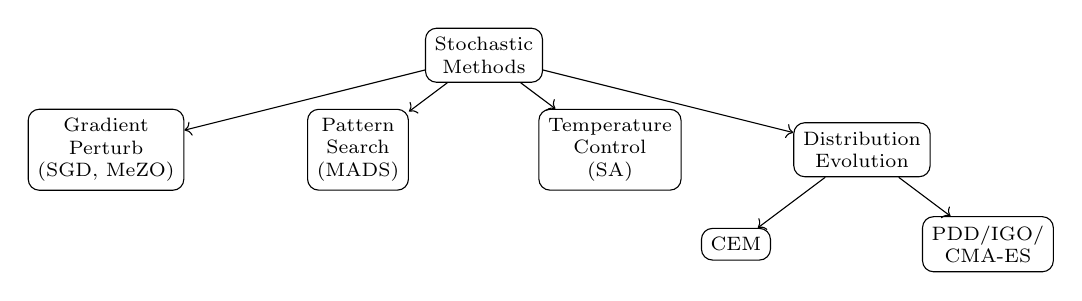
\begin{tikzpicture}[
  every node/.style={draw, rounded corners, align=center, font=\scriptsize},
  edge from parent/.style={draw, ->},
  level distance=1.2cm,
  sibling distance=3.2cm]
\node {Stochastic\\ Methods}
  child { node {Gradient\\ Perturb\\(SGD, MeZO)} }
  child { node {Pattern\\ Search\\(MADS)} }
  child { node {Temperature\\ Control\\(SA)} }
  child { node {Distribution\\ Evolution}
    child { node {CEM} }
    child { node {PDD/IGO/\\CMA-ES} }
  };
\end{tikzpicture}
\end{center}
\end{block}

\begin{block}{Looking Ahead: Chapter 9}
Chapter 9 extends these ideas to \emph{population methods} such as genetic algorithms and particle swarm optimisation.
These methods maintain a diverse \emph{population} of solutions that evolve over time through mechanisms inspired by biological evolution (mutation, crossover, selection) or collective animal behaviour (flocking, swarming).
The distribution-based perspective of Chapter 8 provides the theoretical foundation for understanding why population methods work.
\end{block}

\end{frame}

\end{document}
